%%%%%%%%%%%%%%%%%%%%%%%%%%%%%%%%%%%%%%%%%%%%%%%%%%%%%%%%%%%%%%%%%%%%%%
% Overleaf (WriteLaTeX) Example: Molecular Chemistry Presentation
%
% Source: http://www.overleaf.com
%
% In these slides we show how Overleaf can be used with standard
% chemistry packages to easily create professional presentations.
%
% Feel free to distribute this example, but please keep the referral
% to overleaf.com
%
%%%%%%%%%%%%%%%%%%%%%%%%%%%%%%%%%%%%%%%%%%%%%%%%%%%%%%%%%%%%%%%%%%%%%%

\documentclass[xcolor={dvipsnames}]{beamer}

\mode<presentation>
{
  \usetheme{Madrid}       % or try default, Darmstadt, Warsaw, ...
  \usecolortheme{default} % or try albatross, beaver, crane, ...
  \usefonttheme{default}    % or try default, structurebold, ...
  \setbeamertemplate{navigation symbols}{}
  \setbeamertemplate{caption}[numbered]
}

\usepackage[english]{babel}
\usepackage[utf8x]{inputenc}
\usepackage{graphicx}
\usepackage{hyperref}
  \hypersetup{colorlinks=true}
  \hypersetup{urlcolor=blue}
  \hypersetup{linkcolor = .}
\usepackage{xcolor}
\usepackage{siunitx}
  \sisetup{separate-uncertainty = true}
\DeclareSIUnit\barn{b}
\usepackage{physics}
\usepackage[font=small,labelfont=bf]{caption}
\usepackage{subcaption}
\usepackage[en-GB]{datetime2}
\usepackage{overpic}
\usepackage{feynmp}
\DeclareGraphicsRule{*}{mps}{*}{}
\usepackage{scalerel}
\newcommand{\mylbrace}[2]{\vspace{#2pt}\hspace{6pt}\scaleleftright[\dimexpr5pt+#1\dimexpr0.06pt]{\lbrace}{\rule[\dimexpr2pt-#1\dimexpr0.5pt]{-4pt}{#1pt}}{.}}
\newcommand{\myrbrace}[2]{\vspace{#2pt}\scaleleftright[\dimexpr5pt+#1\dimexpr0.06pt]{.}{\rule[\dimexpr2pt-#1\dimexpr0.5pt]{-4pt}{#1pt}}{\rbrace}\hspace{6pt}}

% Trim in percent
\usepackage{adjustbox}

% No "Figure" prefix
\setbeamertemplate{caption}{\raggedright\insertcaption\par}

% Nice decay amplitude diagrams
\usepackage{amsmath,amssymb,tikz-cd}

% Strike out text
\usepackage[normalem]{ulem}

% For figures with text overlay
\usepackage{overpic}

% Arrows
\usepackage{tikz}
\newcommand{\tikzmark}[1]{\tikz[remember picture] \node[coordinate] (#1) {#1};}

% Colourbox with line breaks
\newcommand{\cbox}[2][lime!20]{%
  \colorbox{#1}{\parbox{\dimexpr\linewidth-2\fboxsep}{\strut #2\strut}}%
}

% Vector arrows
\usepackage[pdftex]{pict2e}

% Checkmark symbol
\def\checkmark{\tikz\fill[scale=0.4](0,.35) -- (.25,0) -- (1,.7) -- (.25,.15) -- cycle;}

% Here's where the presentation starts, with the info for the title slide
\title[Tracking efficiency meeting]{Update on 2026 tracking efficiencies \\ (and 2024 systematics)}

\author[Martin Tat]{Martin Tat}
\institute[Heidelberg]{Heidelberg University}
\date{6th October 2026}

\titlegraphic{
\includegraphics[height = 2.3cm]{lhcb.jpg}\hspace{1.0cm}~%
              
\includegraphics[height = 2.3cm]{HeidelbergLogo.pdf}}

\begin{document}

\begin{frame}
  \titlepage
\end{frame}

% These three lines create an automatically generated table of contents.
%\begin{frame}{Outline}
%  \tableofcontents
%\end{frame}

\begin{frame}{Progress update}
  \vspace{0.0cm}
  {\large Progress update:}
  \vspace{0.2cm}
  \begin{enumerate}
    \setlength\itemsep{0.8em}
    \item{2026 efficiencies calculated in 1D using expected MC}
    \begin{itemize}
      \item[-]{2D tables could easily be produced...}
      \item[-]{... but is this needed?}
    \end{itemize}
    \item{2024 analysis:}
    \begin{itemize}
      \item[\checkmark]{Data/MC tupling of 24r2 successful}
      \item[\checkmark]{Reweighting working}
      \item[-]{Need to retuple data with CONDITIONAL runs}
      \item[-]{Systematics considered: Multiplicity reweighting, mass shape, Combined-MuonUT discrepancy}
      \item[-]{Separate tables for $\mu^+$, $\mu^-$, $\mu^\pm$}
    \end{itemize}
  \end{enumerate}
\end{frame}

\begin{frame}{2026 tracking efficiencies}
  \vspace{0.0cm}
  {\large Comparison of tracking efficiencies in 2026 data blocks}
  \begin{figure}[htb]
    \centering
    \begin{subfigure}{0.5\textwidth}
      \centering
      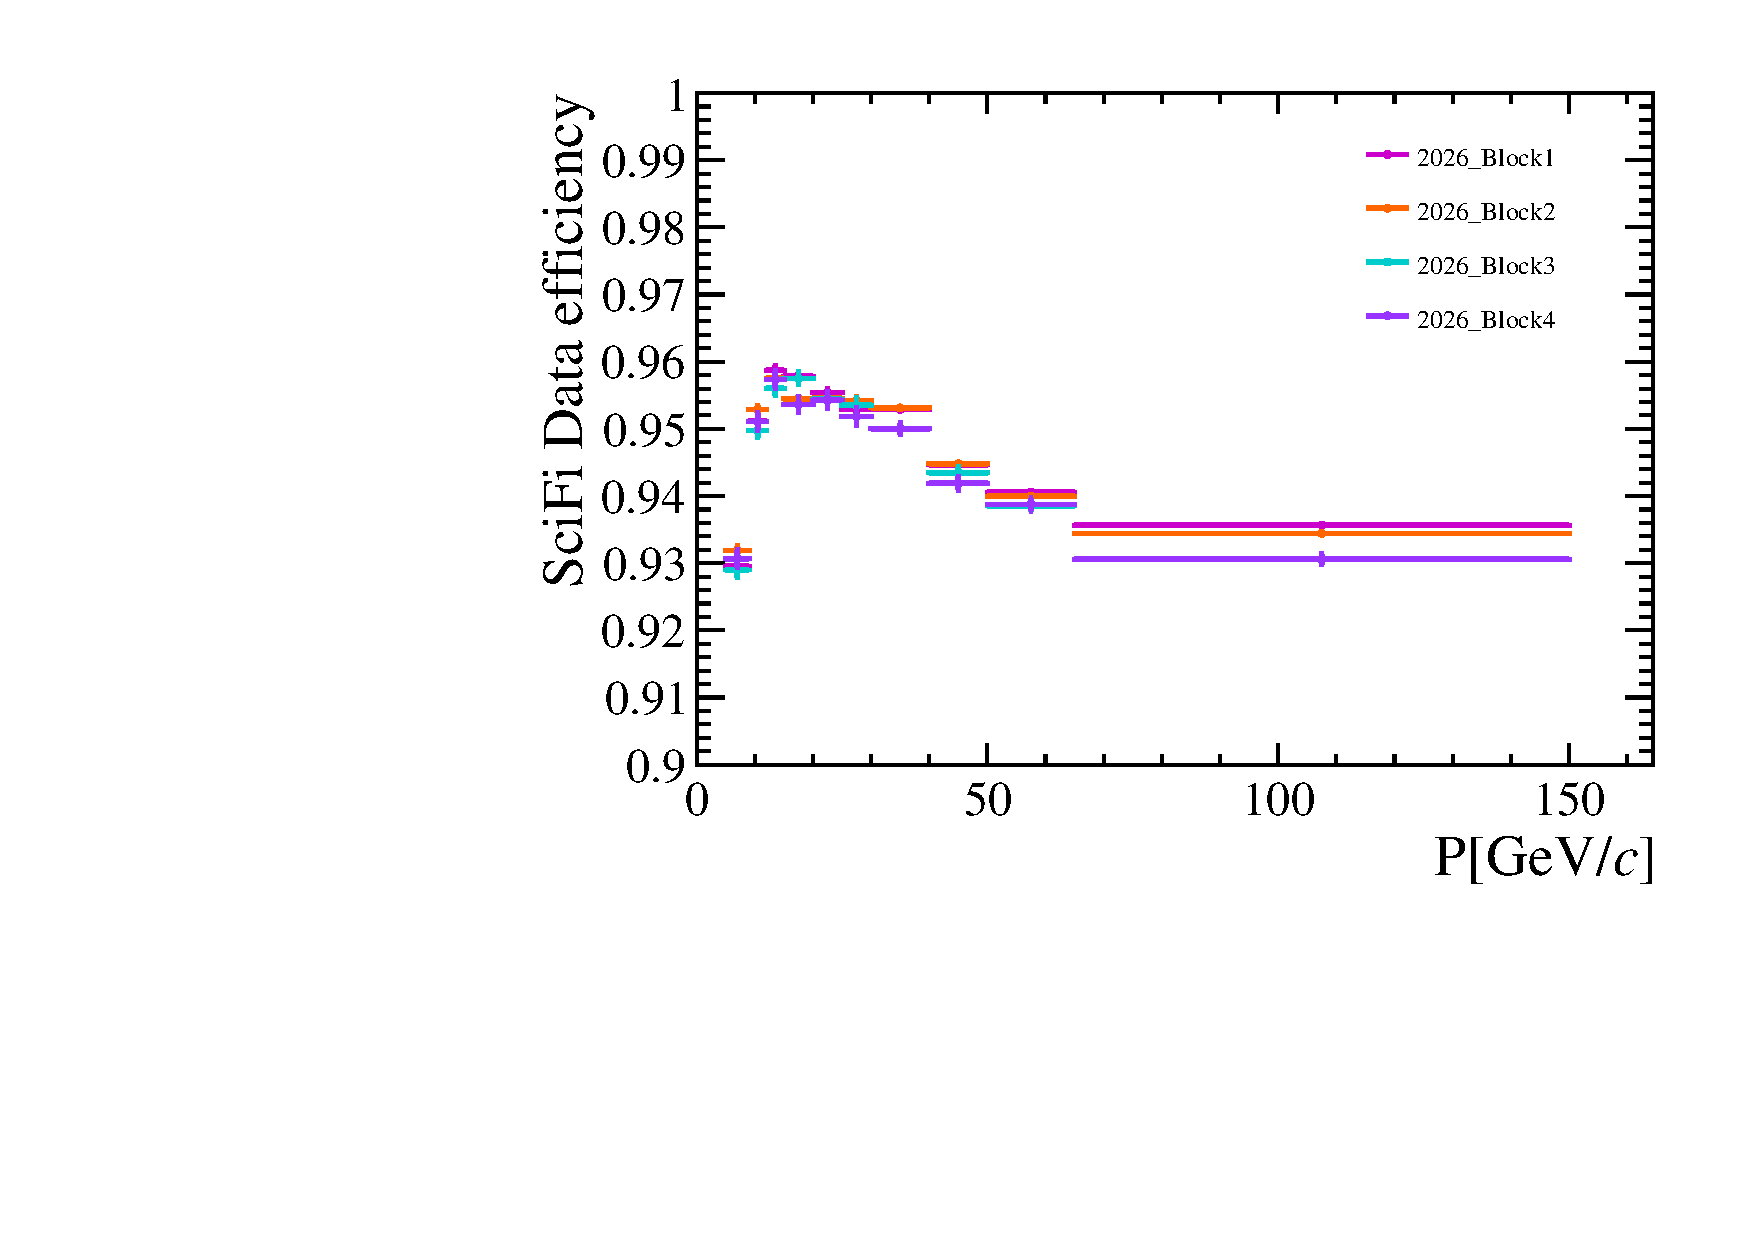
\includegraphics[width=1.0\textwidth]{Plots/trackeff_Data_VeloMuon_P_2026_expected_MC_samples.pdf}
    \end{subfigure}%
    \begin{subfigure}{0.5\textwidth}
      \centering
      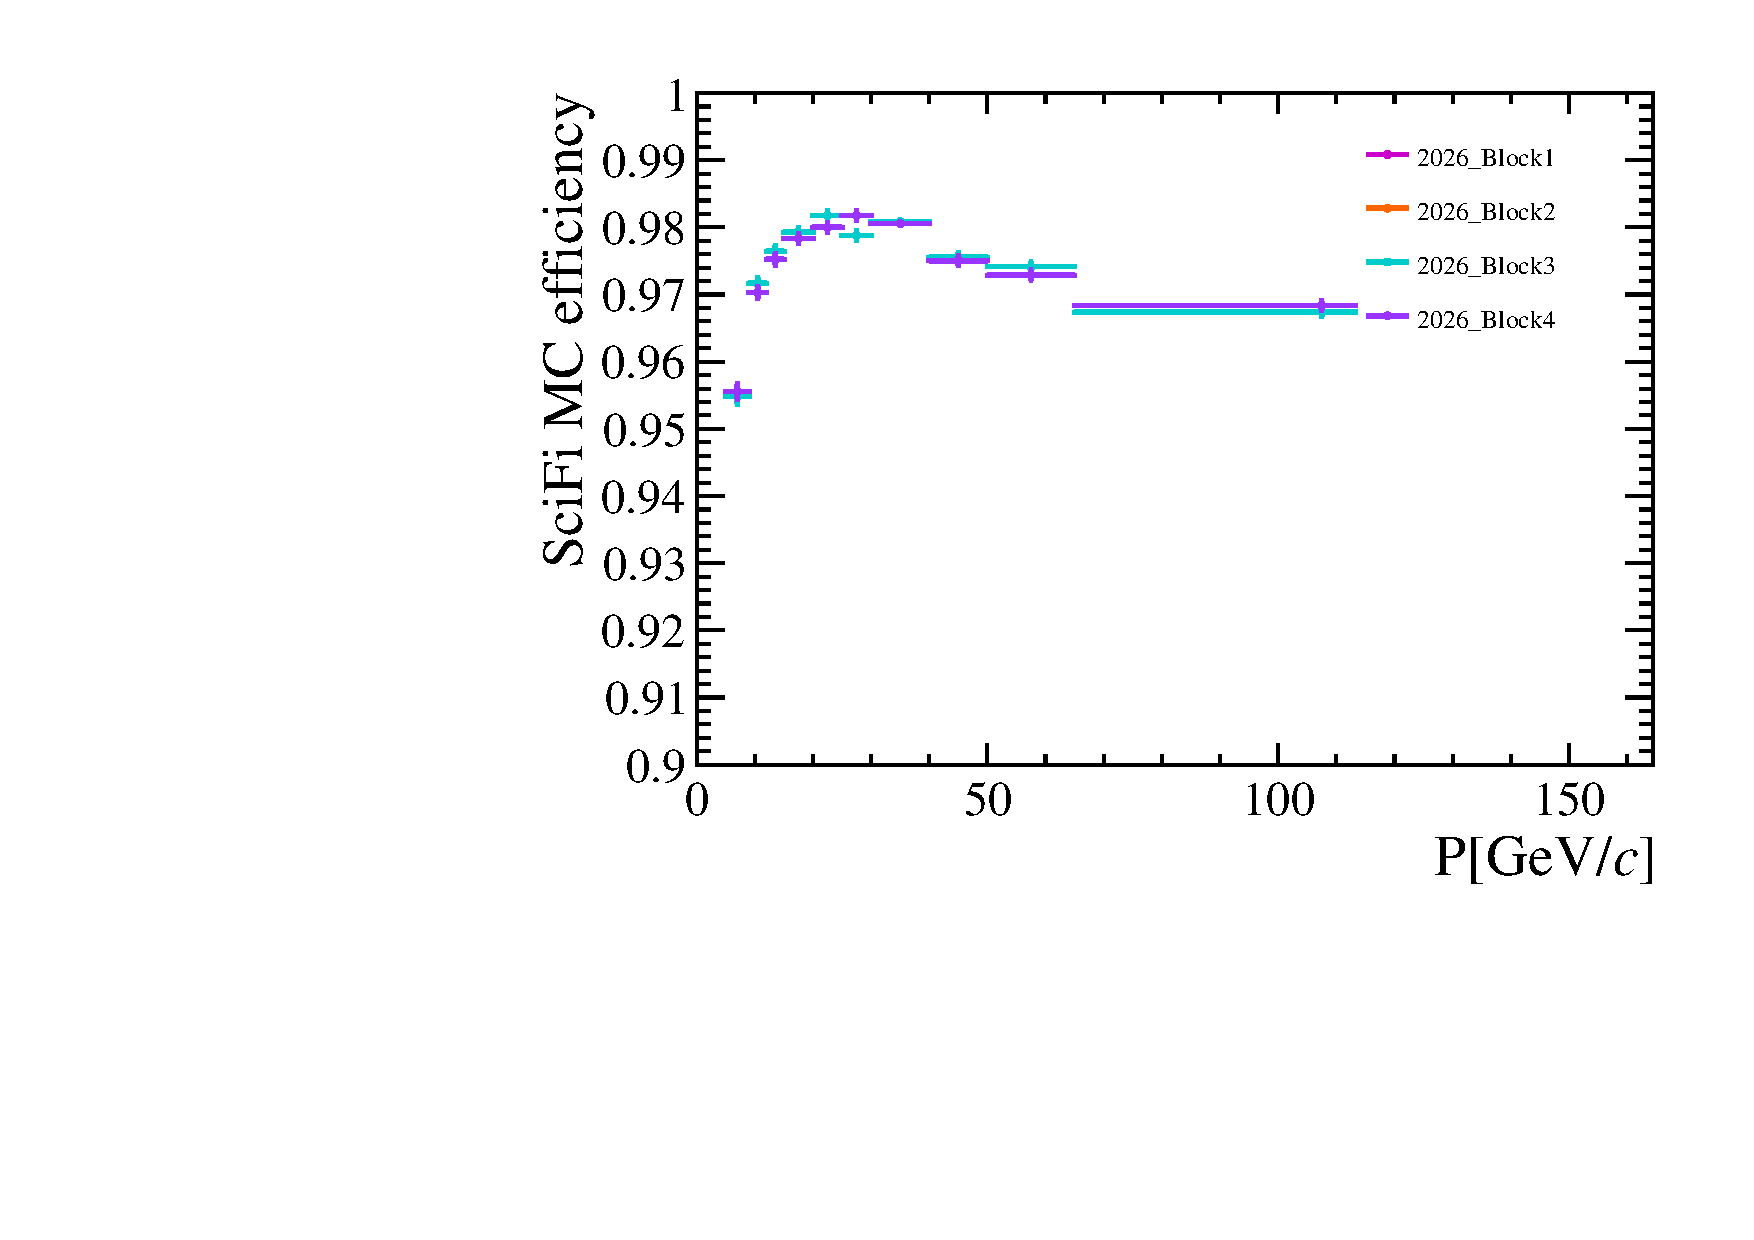
\includegraphics[width=1.0\textwidth]{Plots/trackeff_MC_VeloMuon_P_2026_expected_MC_samples.pdf}
    \end{subfigure}
  \end{figure}
  {SciFi efficiencies looks quite different between data and MC...}
\end{frame}

\begin{frame}{2026 tracking efficiencies}
  \vspace{0.0cm}
  {\large Comparison of tracking efficiencies in 2026 data blocks}
  \begin{figure}[htb]
    \centering
    \begin{subfigure}{0.5\textwidth}
      \centering
      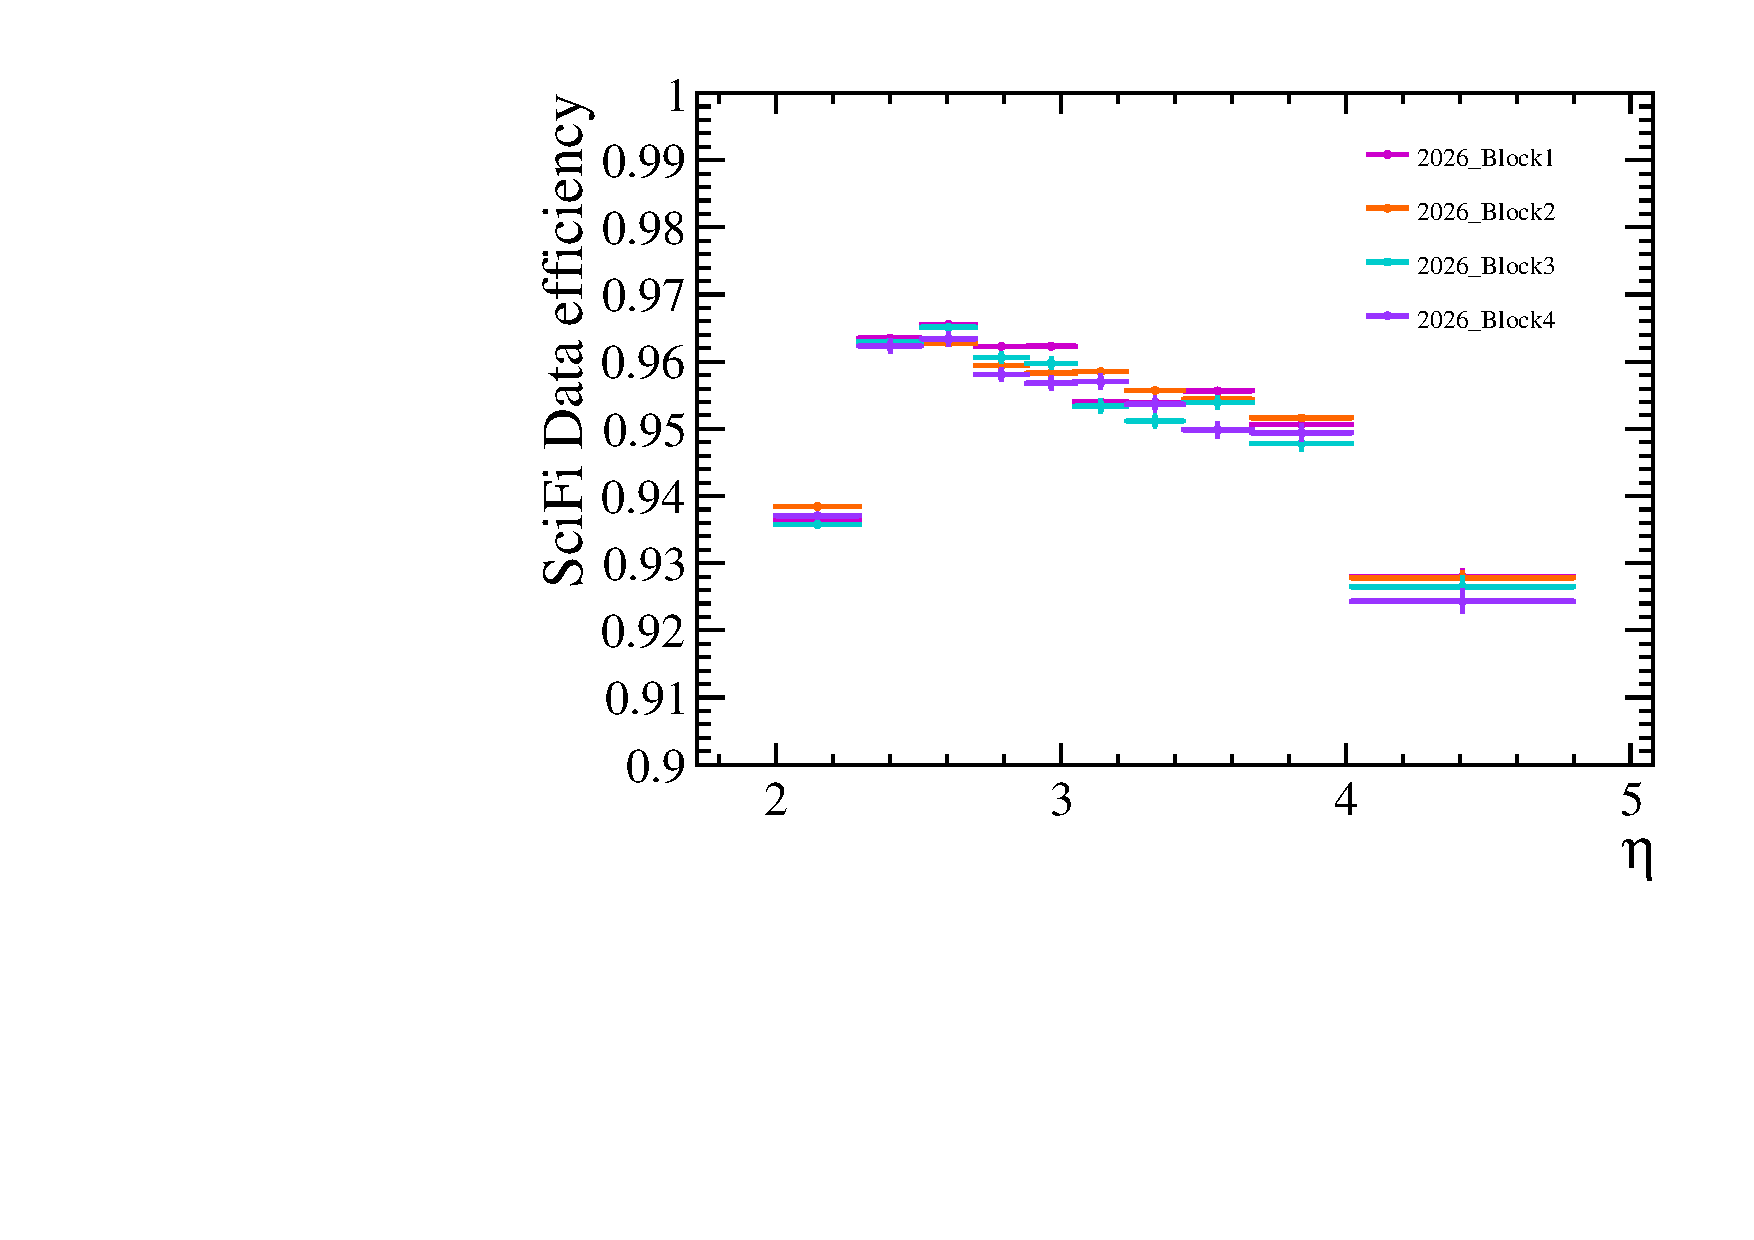
\includegraphics[width=1.0\textwidth]{Plots/trackeff_Data_VeloMuon_ETA_2026_expected_MC_samples.pdf}
    \end{subfigure}%
    \begin{subfigure}{0.5\textwidth}
      \centering
      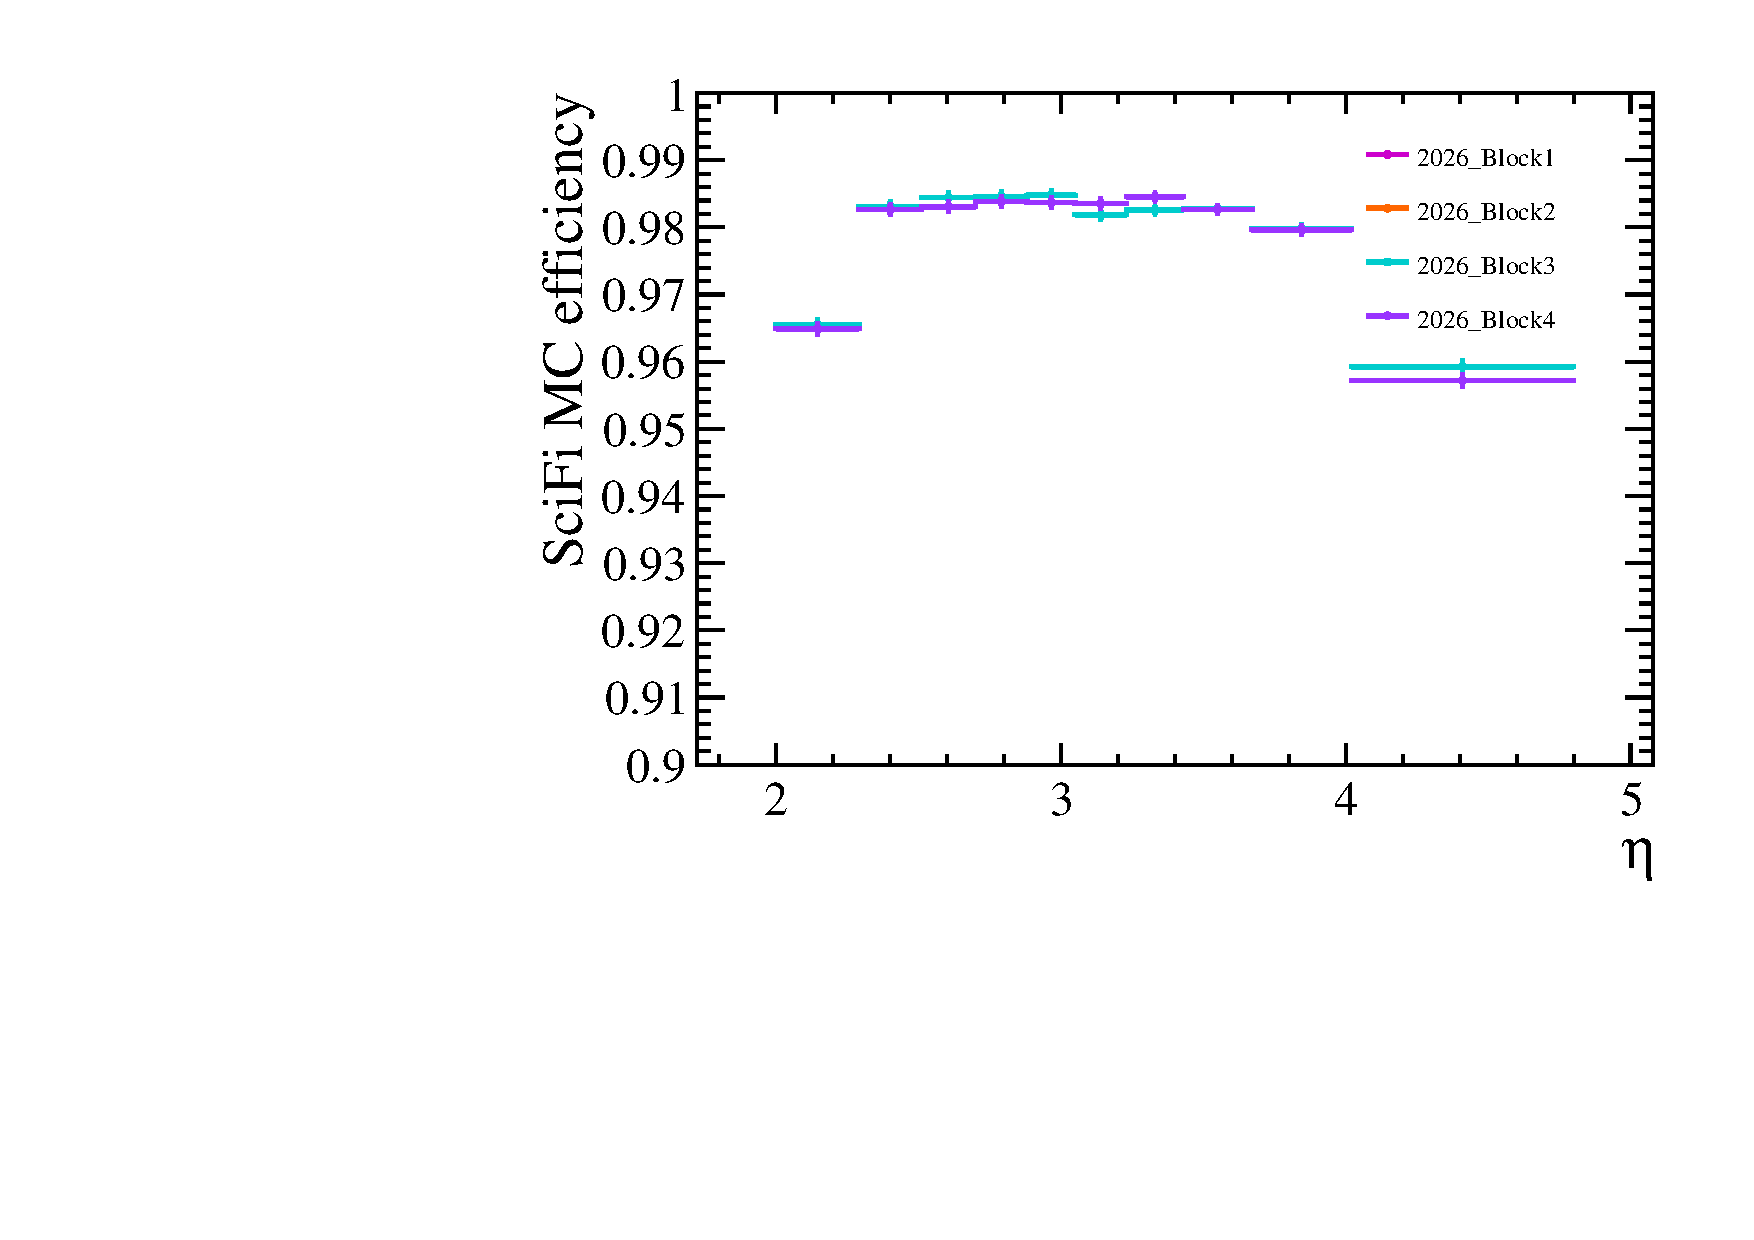
\includegraphics[width=1.0\textwidth]{Plots/trackeff_MC_VeloMuon_ETA_2026_expected_MC_samples.pdf}
    \end{subfigure}
  \end{figure}
  {SciFi efficiencies looks quite different between data and MC...}
\end{frame}

\begin{frame}{2026 tracking efficiencies}
  \vspace{0.0cm}
  {\large Comparison of tracking efficiencies in 2026 data blocks}
  \begin{figure}[htb]
    \centering
    \begin{subfigure}{0.5\textwidth}
      \centering
      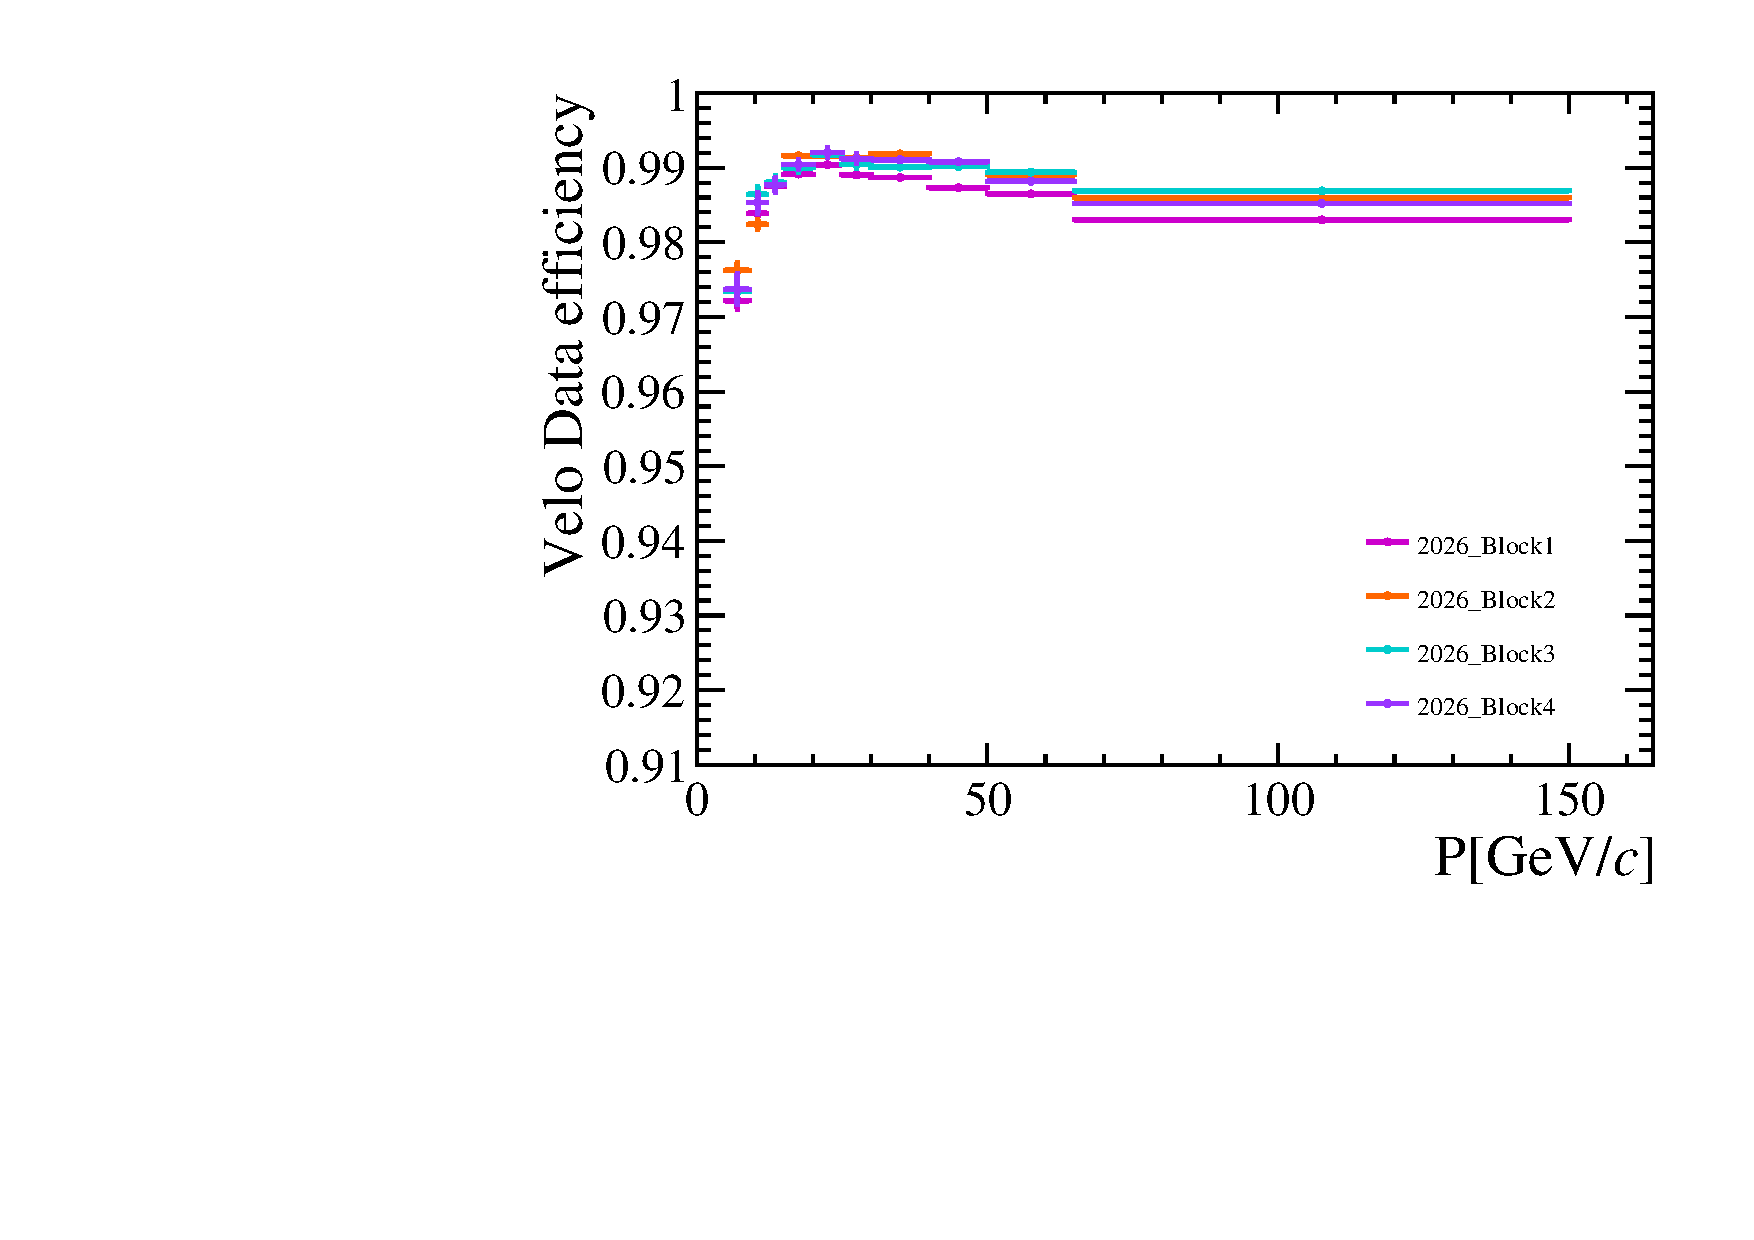
\includegraphics[width=1.0\textwidth]{Plots/trackeff_Data_Downstream_P_2026_expected_MC_samples.pdf}
    \end{subfigure}%
    \begin{subfigure}{0.5\textwidth}
      \centering
      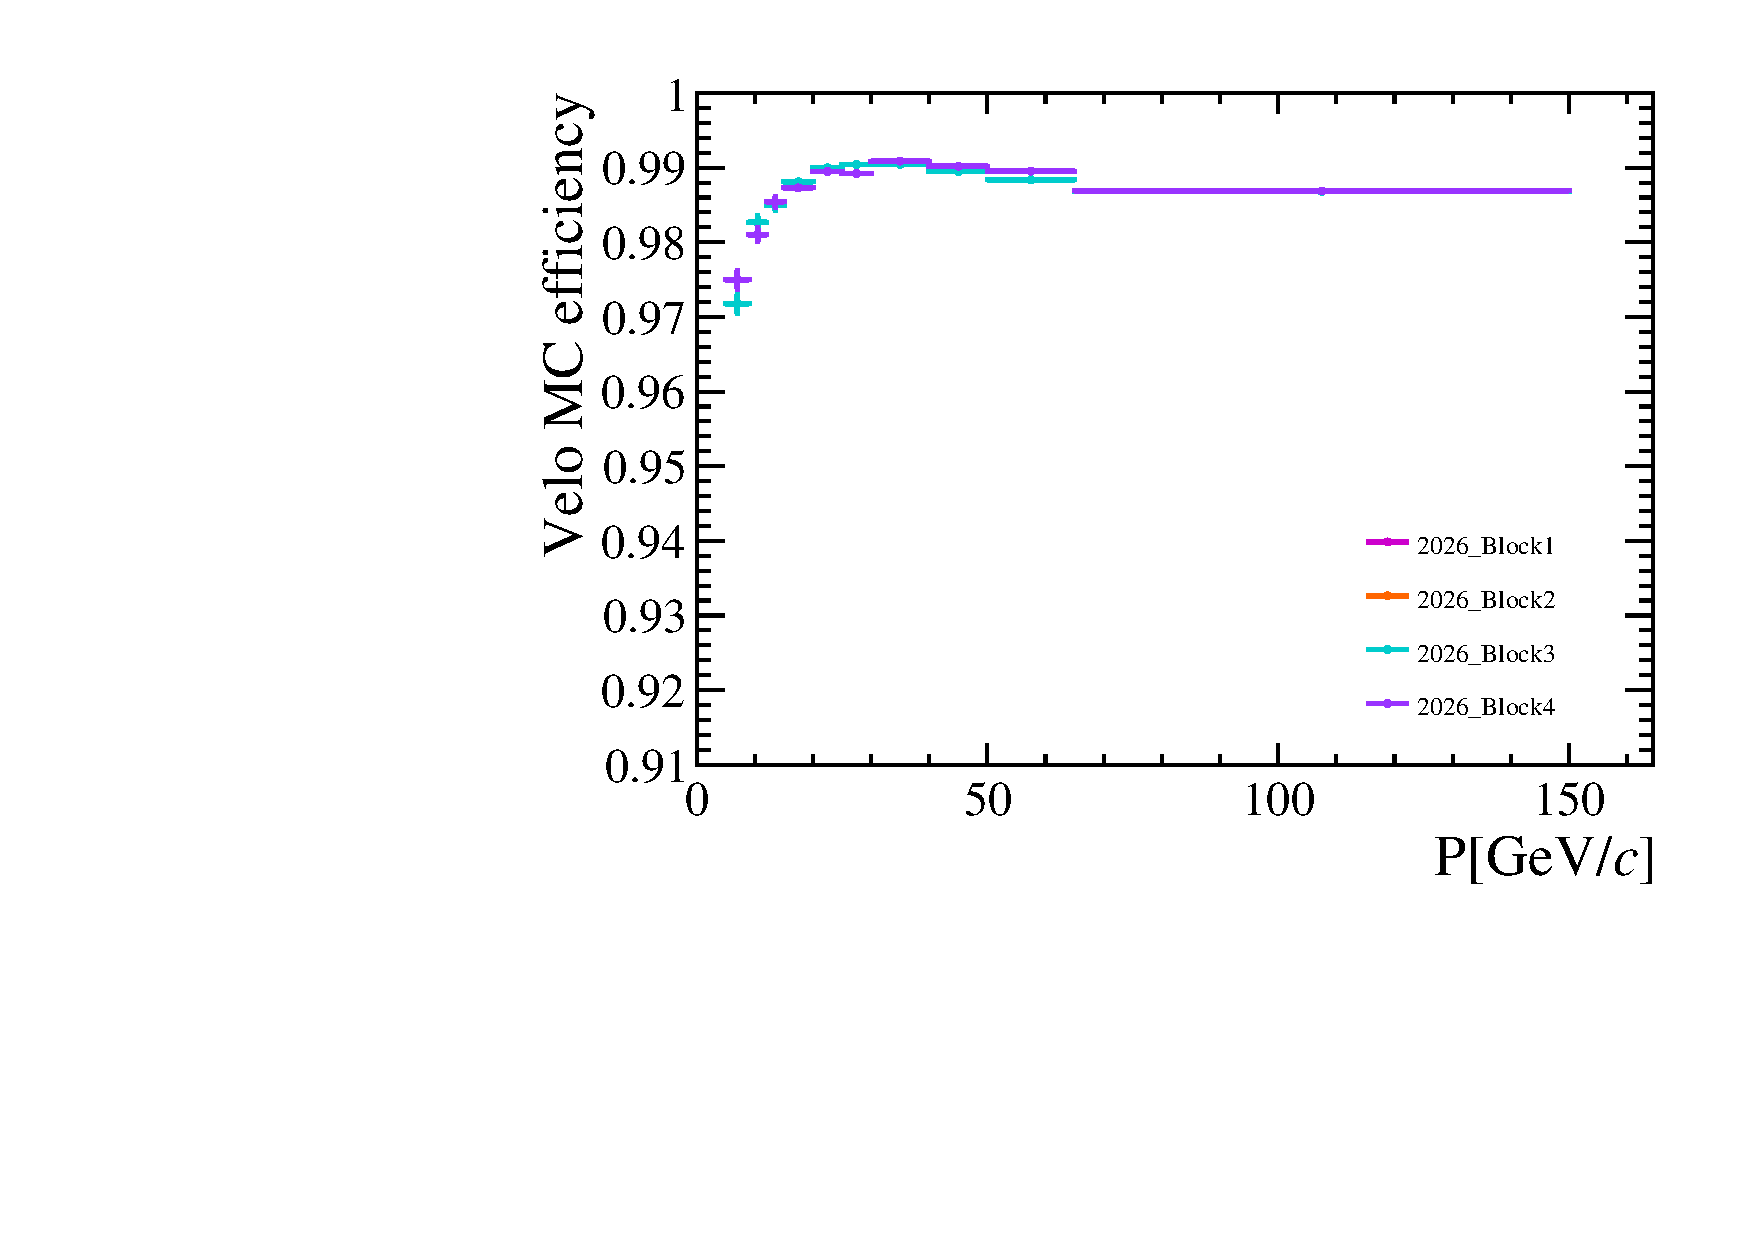
\includegraphics[width=1.0\textwidth]{Plots/trackeff_MC_Downstream_P_2026_expected_MC_samples.pdf}
    \end{subfigure}
  \end{figure}
  {Velo efficiencies agree reasonably well between data and MC...}
\end{frame}

\begin{frame}{2026 tracking efficiencies}
  \vspace{0.0cm}
  {\large Comparison of tracking efficiencies in 2026 data blocks}
  \begin{figure}[htb]
    \centering
    \begin{subfigure}{0.5\textwidth}
      \centering
      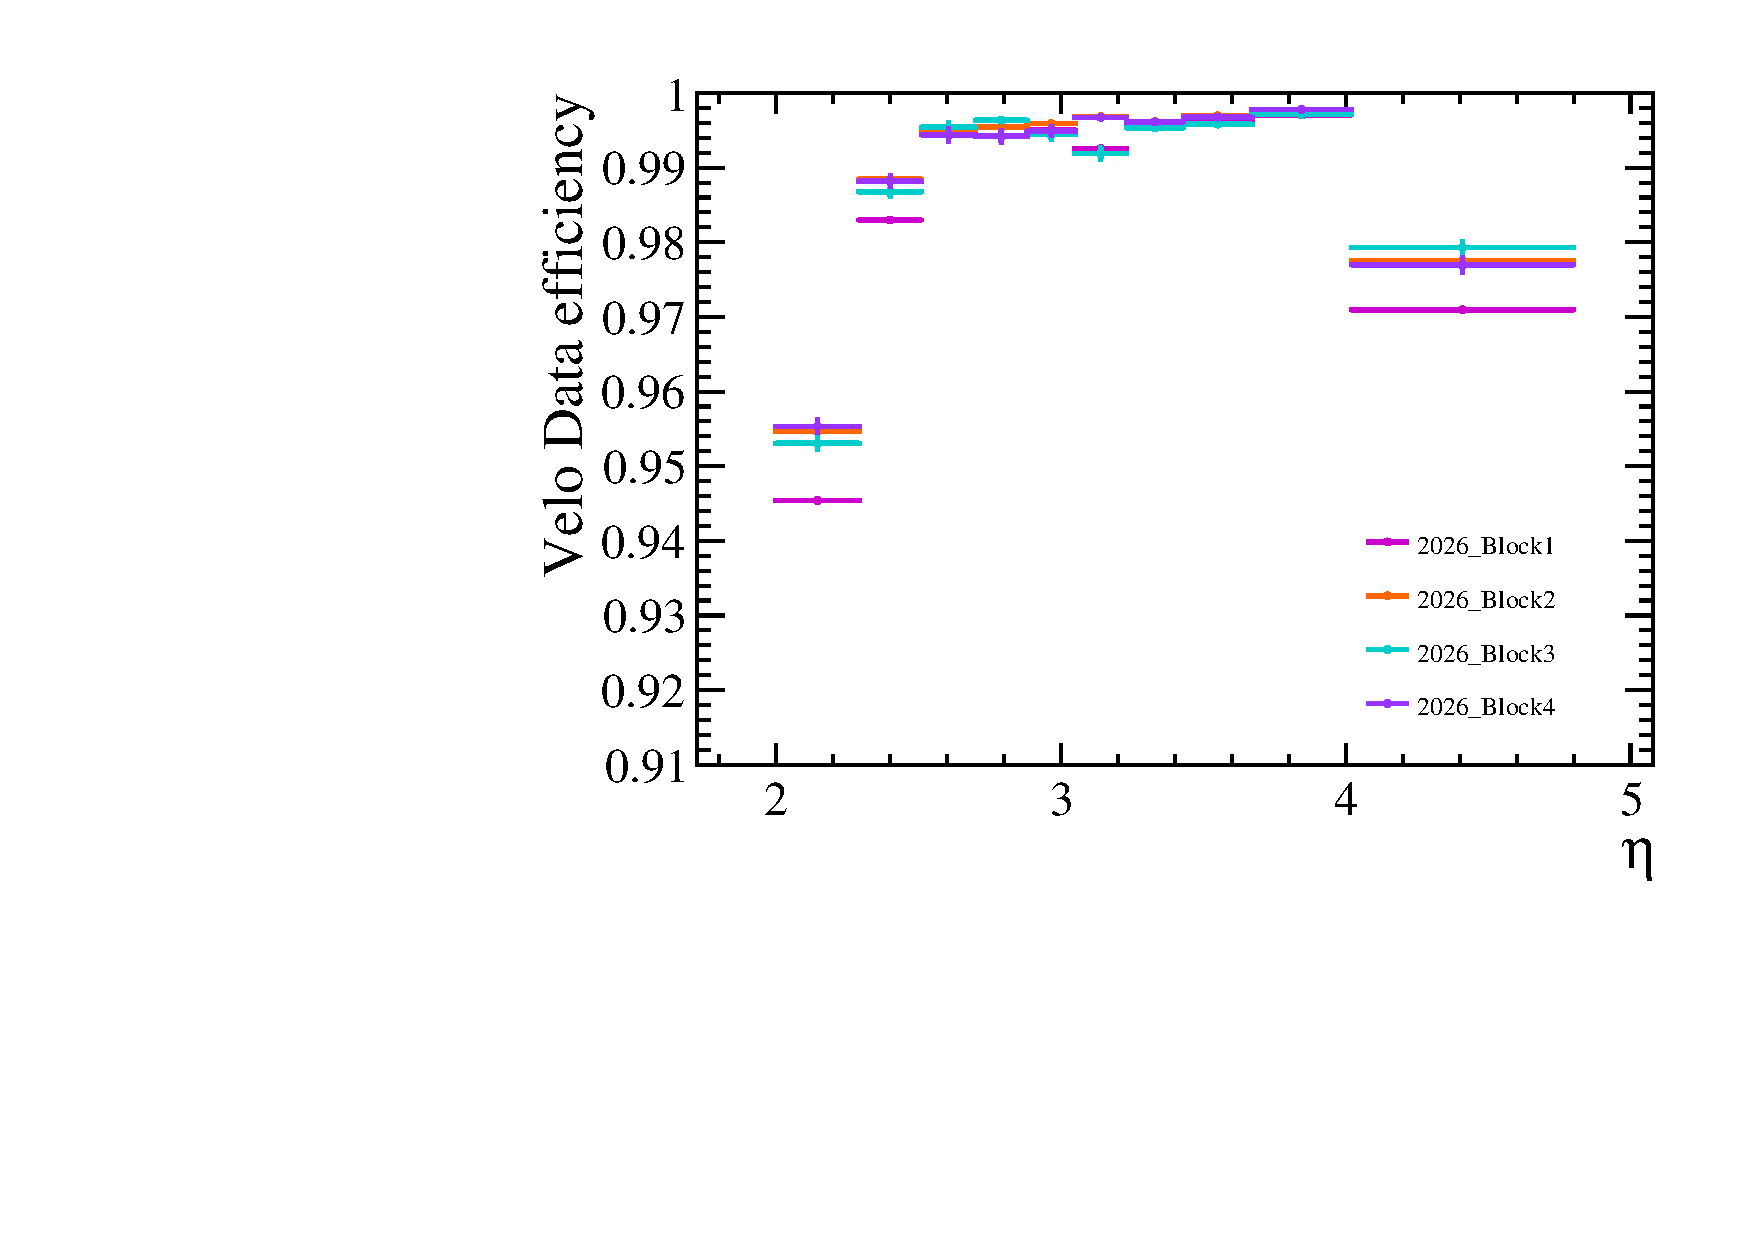
\includegraphics[width=1.0\textwidth]{Plots/trackeff_Data_Downstream_ETA_2026_expected_MC_samples.pdf}
    \end{subfigure}%
    \begin{subfigure}{0.5\textwidth}
      \centering
      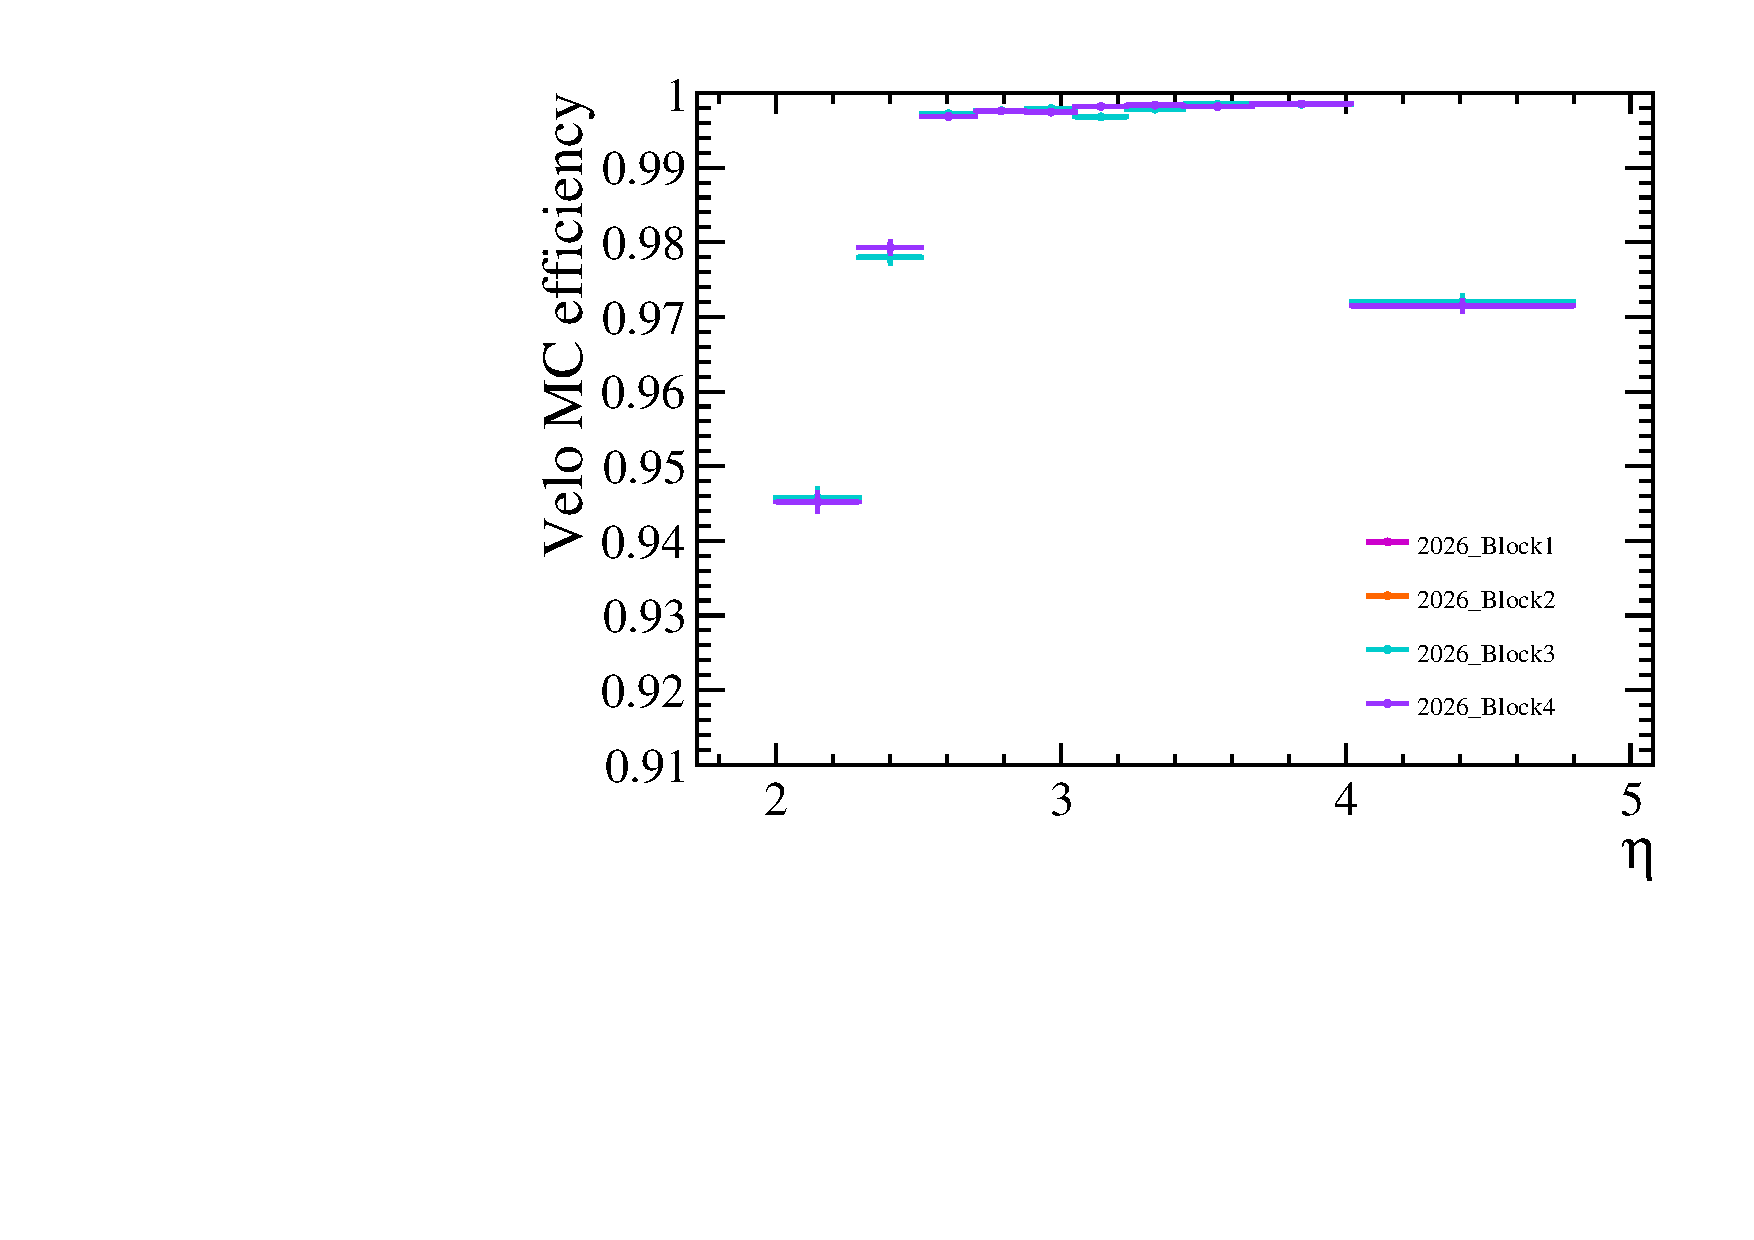
\includegraphics[width=1.0\textwidth]{Plots/trackeff_MC_Downstream_ETA_2026_expected_MC_samples.pdf}
    \end{subfigure}
  \end{figure}
  {Velo efficiencies agree reasonably well between data and MC...}
\end{frame}

\begin{frame}{Velo changes during data taking}
  \vspace{0.0cm}
  \begin{itemize}
    \item{It's unclear why the Velo efficiencies are higher in Blocks 2, 3, 4}
    \item{From Run meeting Velo minutes on 20th March 2026:}
    \begin{itemize}
      \item[-]{``Tuesday. HV recipes updated. STANDBY2 with 400V for inner sensors and 200V for outer sensors. M30 VP2 with 600V at ready''}
    \end{itemize}
    \item{From Run meeting Velo minutes on 24th March 2026:}
    \begin{itemize}
      \item[-]{``HV recipes updated with M30/M31 VP2 and VP0 at 600V''}
      \item[-]{``... After some investigation, M30 VP2-0 was confirmed to be damaged. HV recipes rollback to 400V inner sensors and 200V outer sensors.''}
    \end{itemize}
    \item{Magnet flip happened on 25th March 2026}
    \item{Clearly there were changes to HV settings of the Velo during this period, but it's unclear if this can explain the increase in Velo efficiency at high and low $\eta$, especially since around this period the first failed Velo modules started appearing}
  \end{itemize}
\end{frame}

\begin{frame}{2026 tracking efficiencies}
  \vspace{0.0cm}
  {\large Comparison of tracking efficiencies in 2026 data blocks}
  \begin{figure}[htb]
    \centering
    \begin{subfigure}{0.5\textwidth}
      \centering
      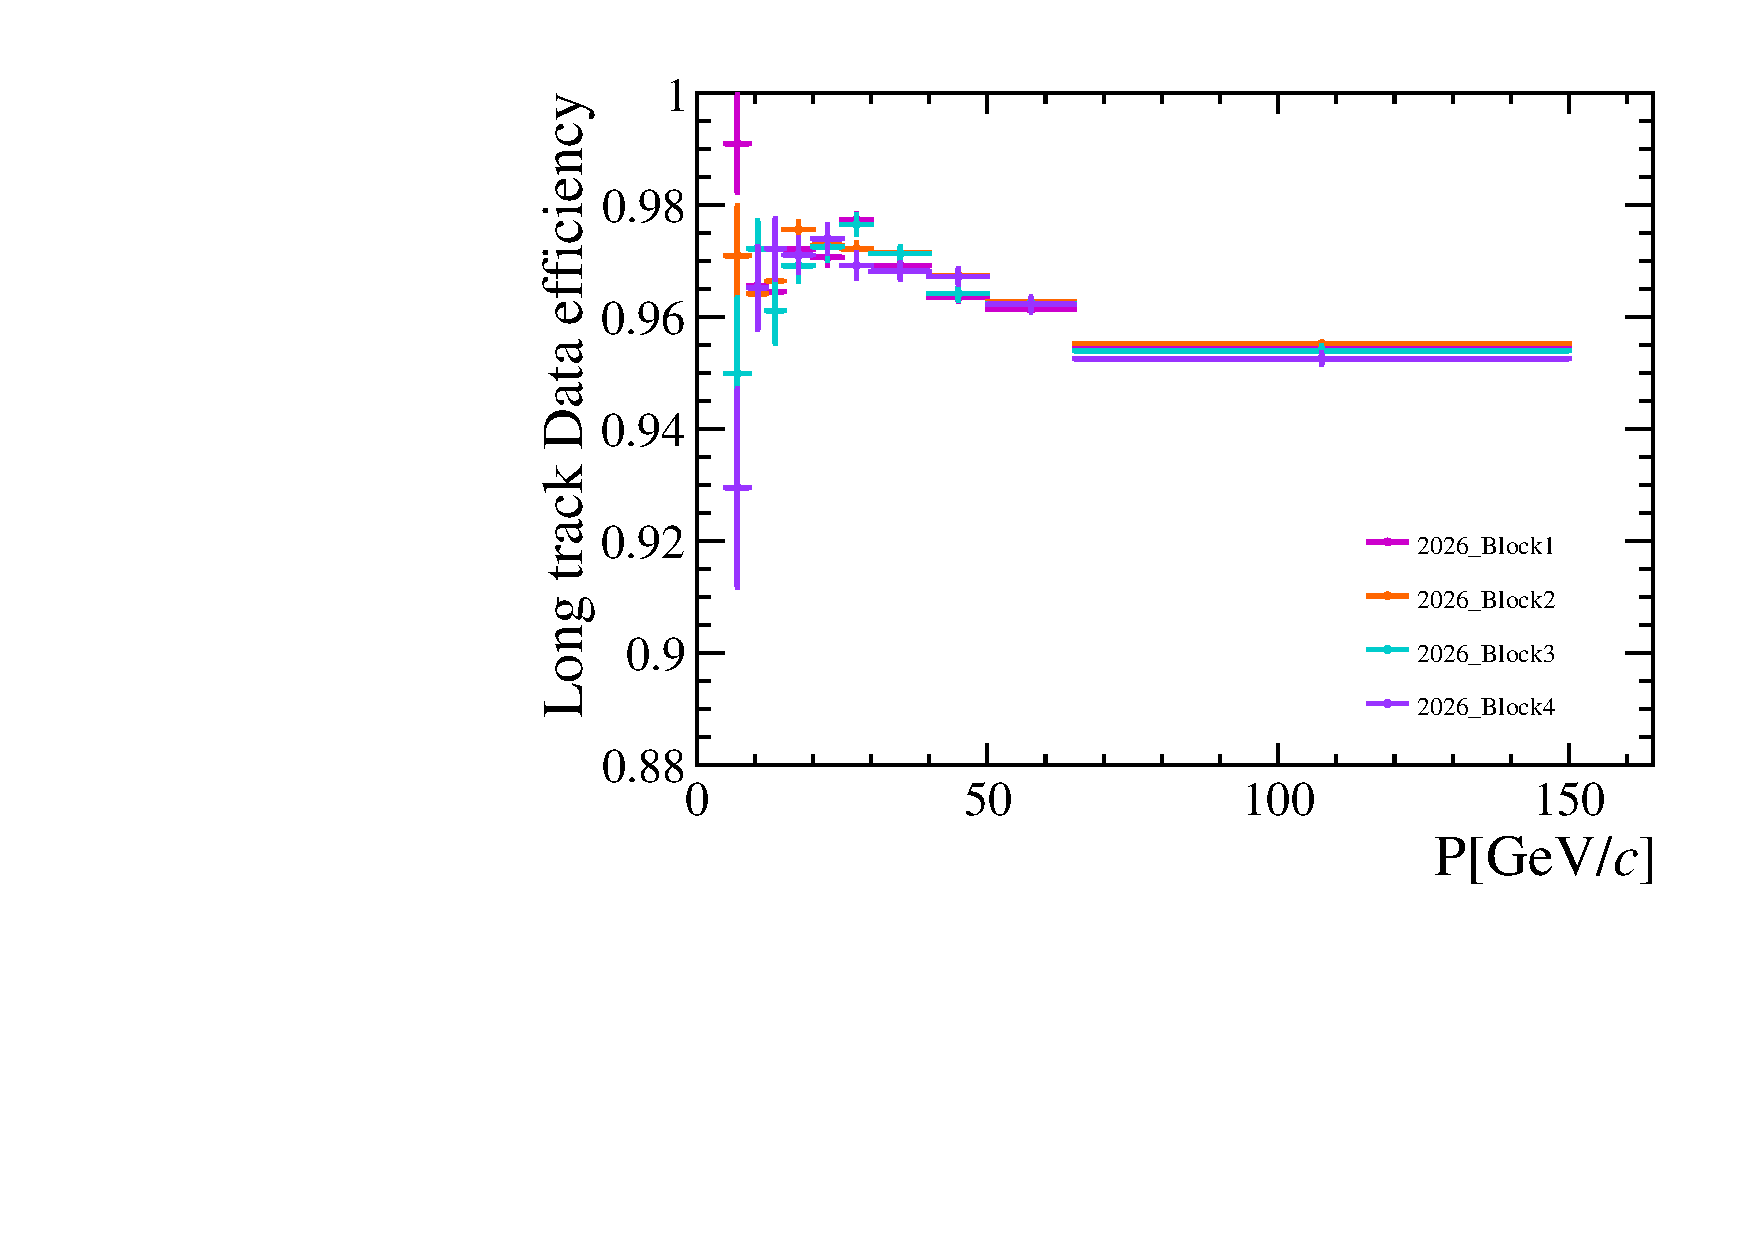
\includegraphics[width=1.0\textwidth]{Plots/trackeff_Data_MuonUT_P_2026_expected_MC_samples.pdf}
    \end{subfigure}%
    \begin{subfigure}{0.5\textwidth}
      \centering
      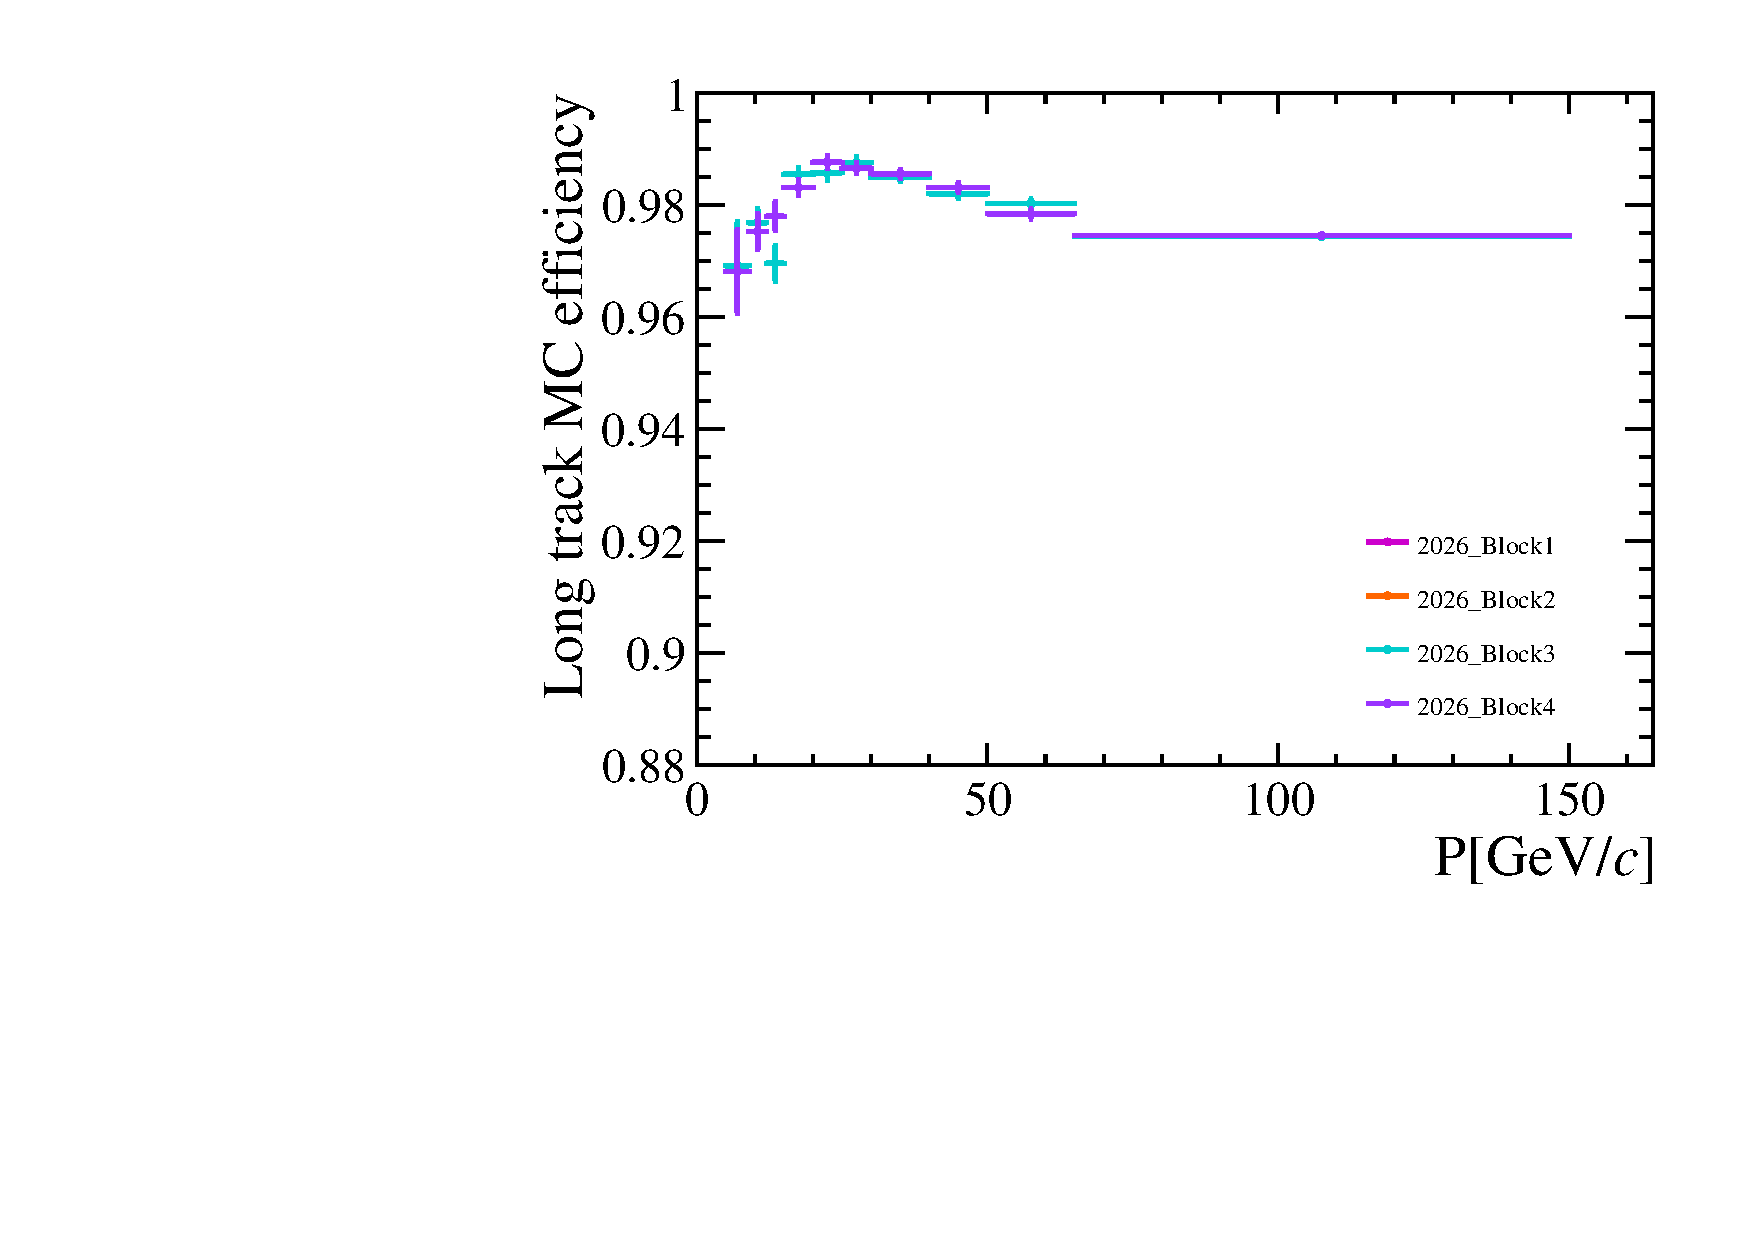
\includegraphics[width=1.0\textwidth]{Plots/trackeff_MC_MuonUT_P_2026_expected_MC_samples.pdf}
    \end{subfigure}
  \end{figure}
  {MuonUT efficiencies have consistent trend between data and MC}
\end{frame}

\begin{frame}{2026 tracking efficiencies}
  \vspace{0.0cm}
  {\large Comparison of tracking efficiencies in 2026 data blocks}
  \begin{figure}[htb]
    \centering
    \begin{subfigure}{0.5\textwidth}
      \centering
      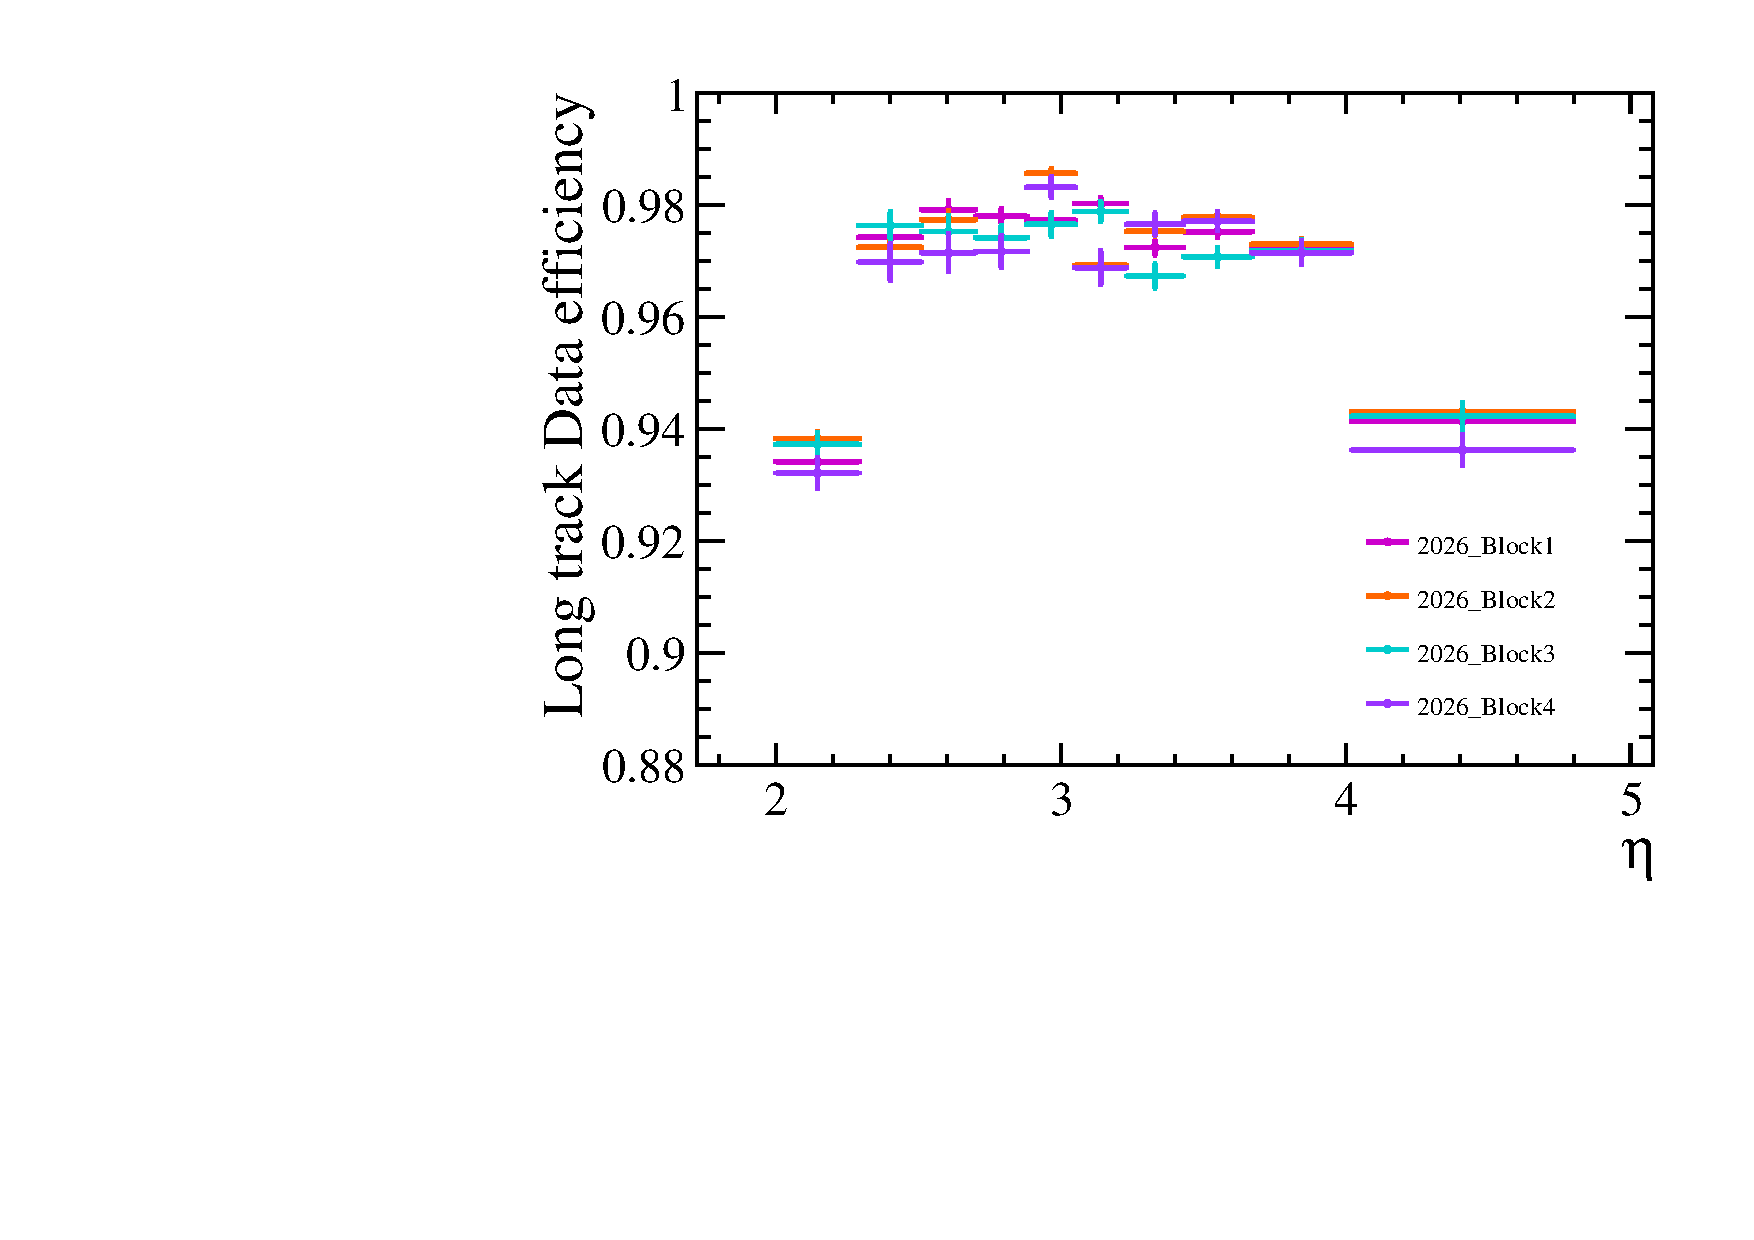
\includegraphics[width=1.0\textwidth]{Plots/trackeff_Data_MuonUT_ETA_2026_expected_MC_samples.pdf}
    \end{subfigure}%
    \begin{subfigure}{0.5\textwidth}
      \centering
      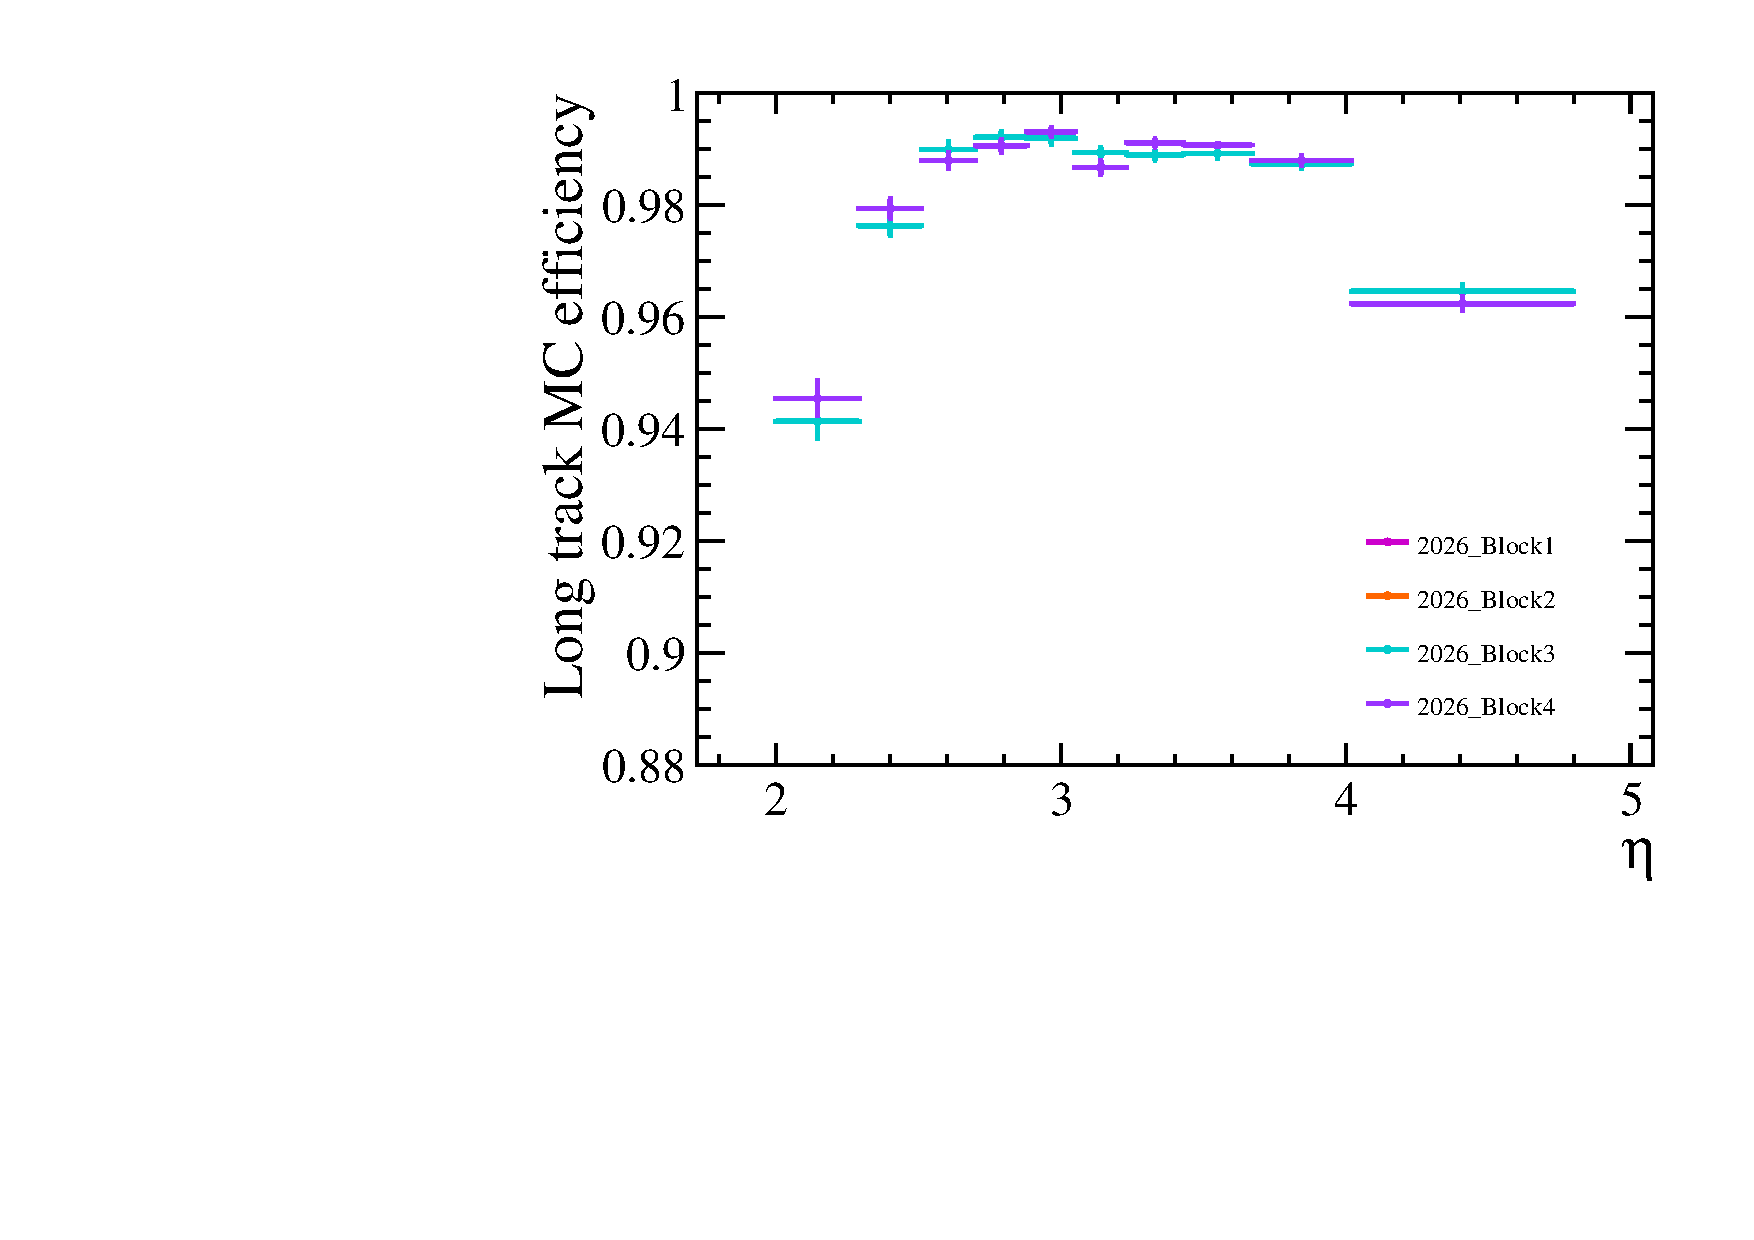
\includegraphics[width=1.0\textwidth]{Plots/trackeff_MC_MuonUT_ETA_2026_expected_MC_samples.pdf}
    \end{subfigure}
  \end{figure}
  {MuonUT efficiencies have consistent trend between data and MC}
\end{frame}

\begin{frame}{2026 tracking efficiency ratios}
  \vspace{0.0cm}
  {\large Comparison of tracking efficiency ratios in 2026 Block 1}
  \begin{figure}[htb]
    \centering
    \begin{subfigure}{0.5\textwidth}
      \centering
      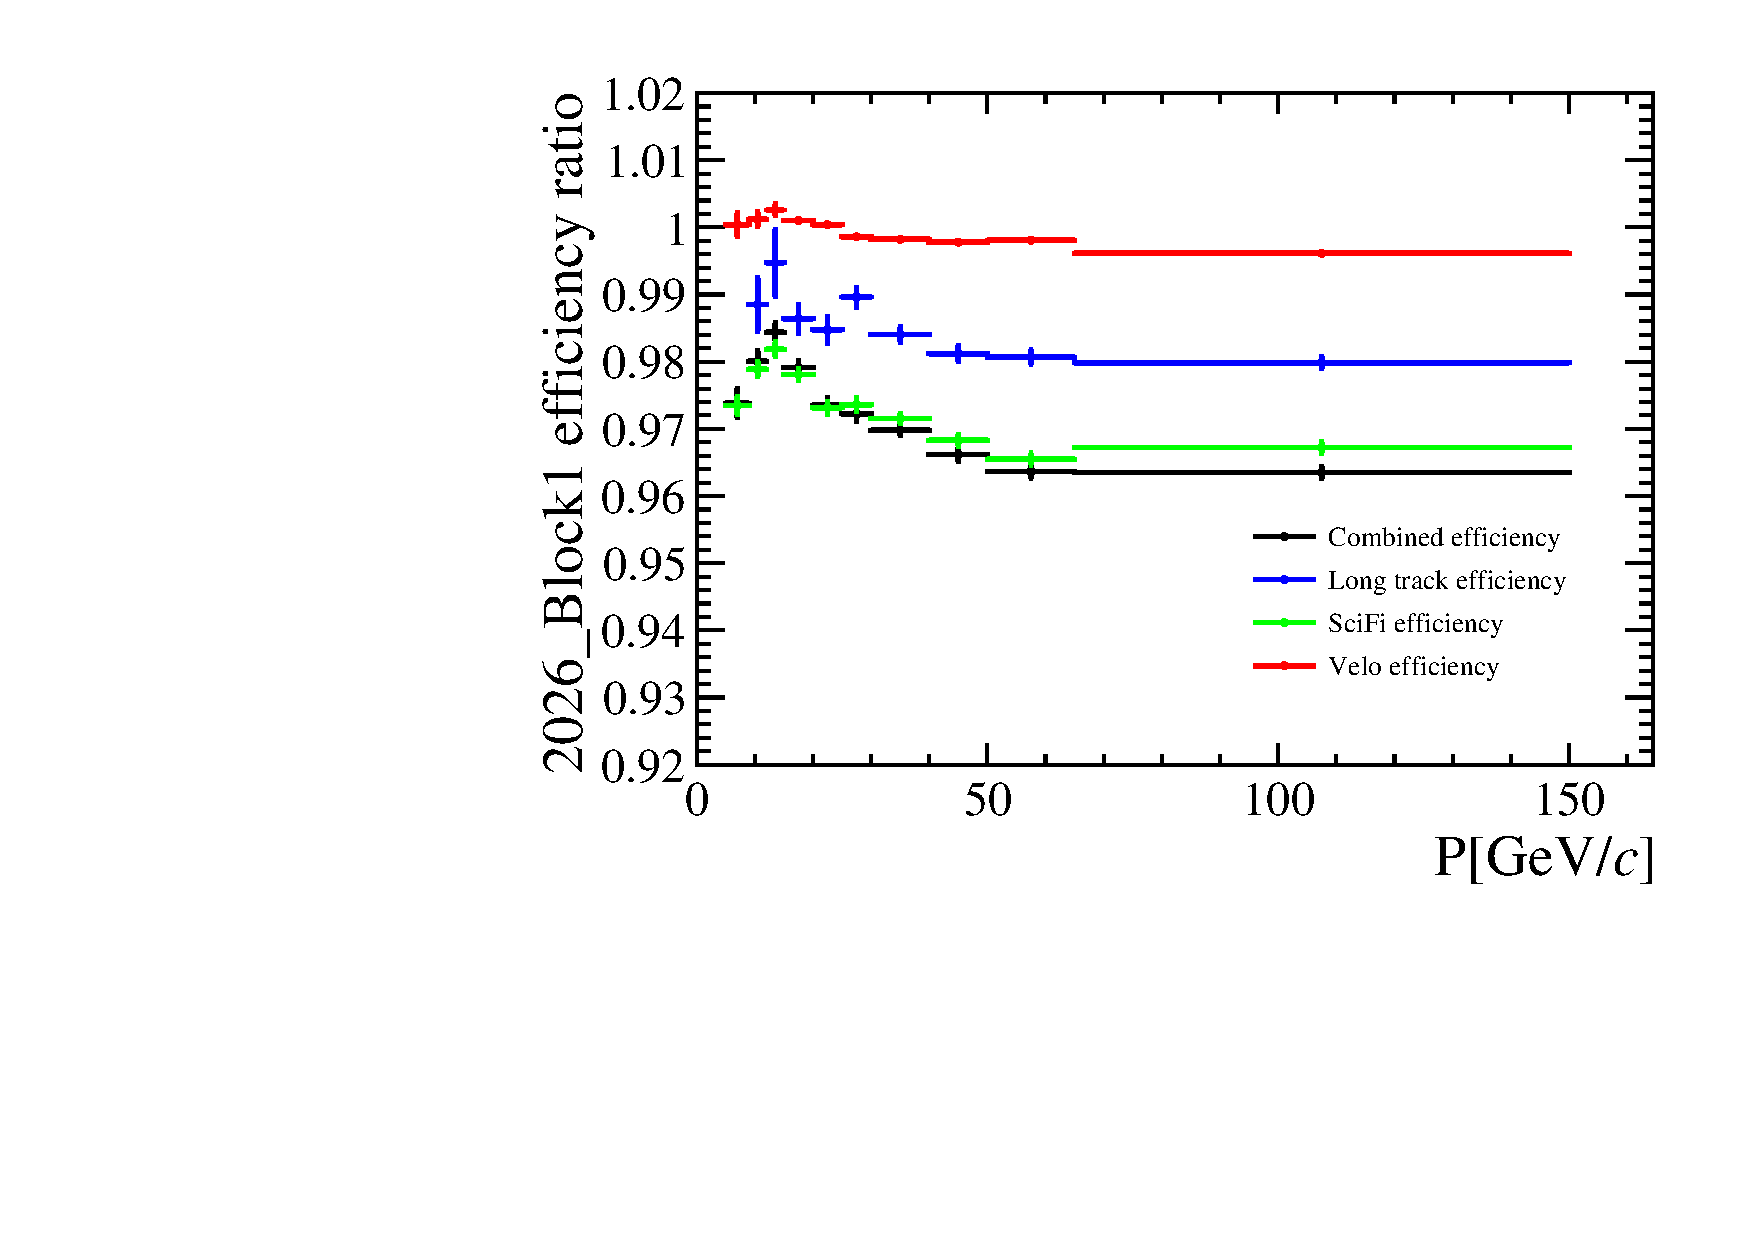
\includegraphics[width=1.0\textwidth]{Plots/trackeff_ratio_P_2026_Block1_2026_expected_MC_samples.pdf}
    \end{subfigure}%
    \begin{subfigure}{0.5\textwidth}
      \centering
      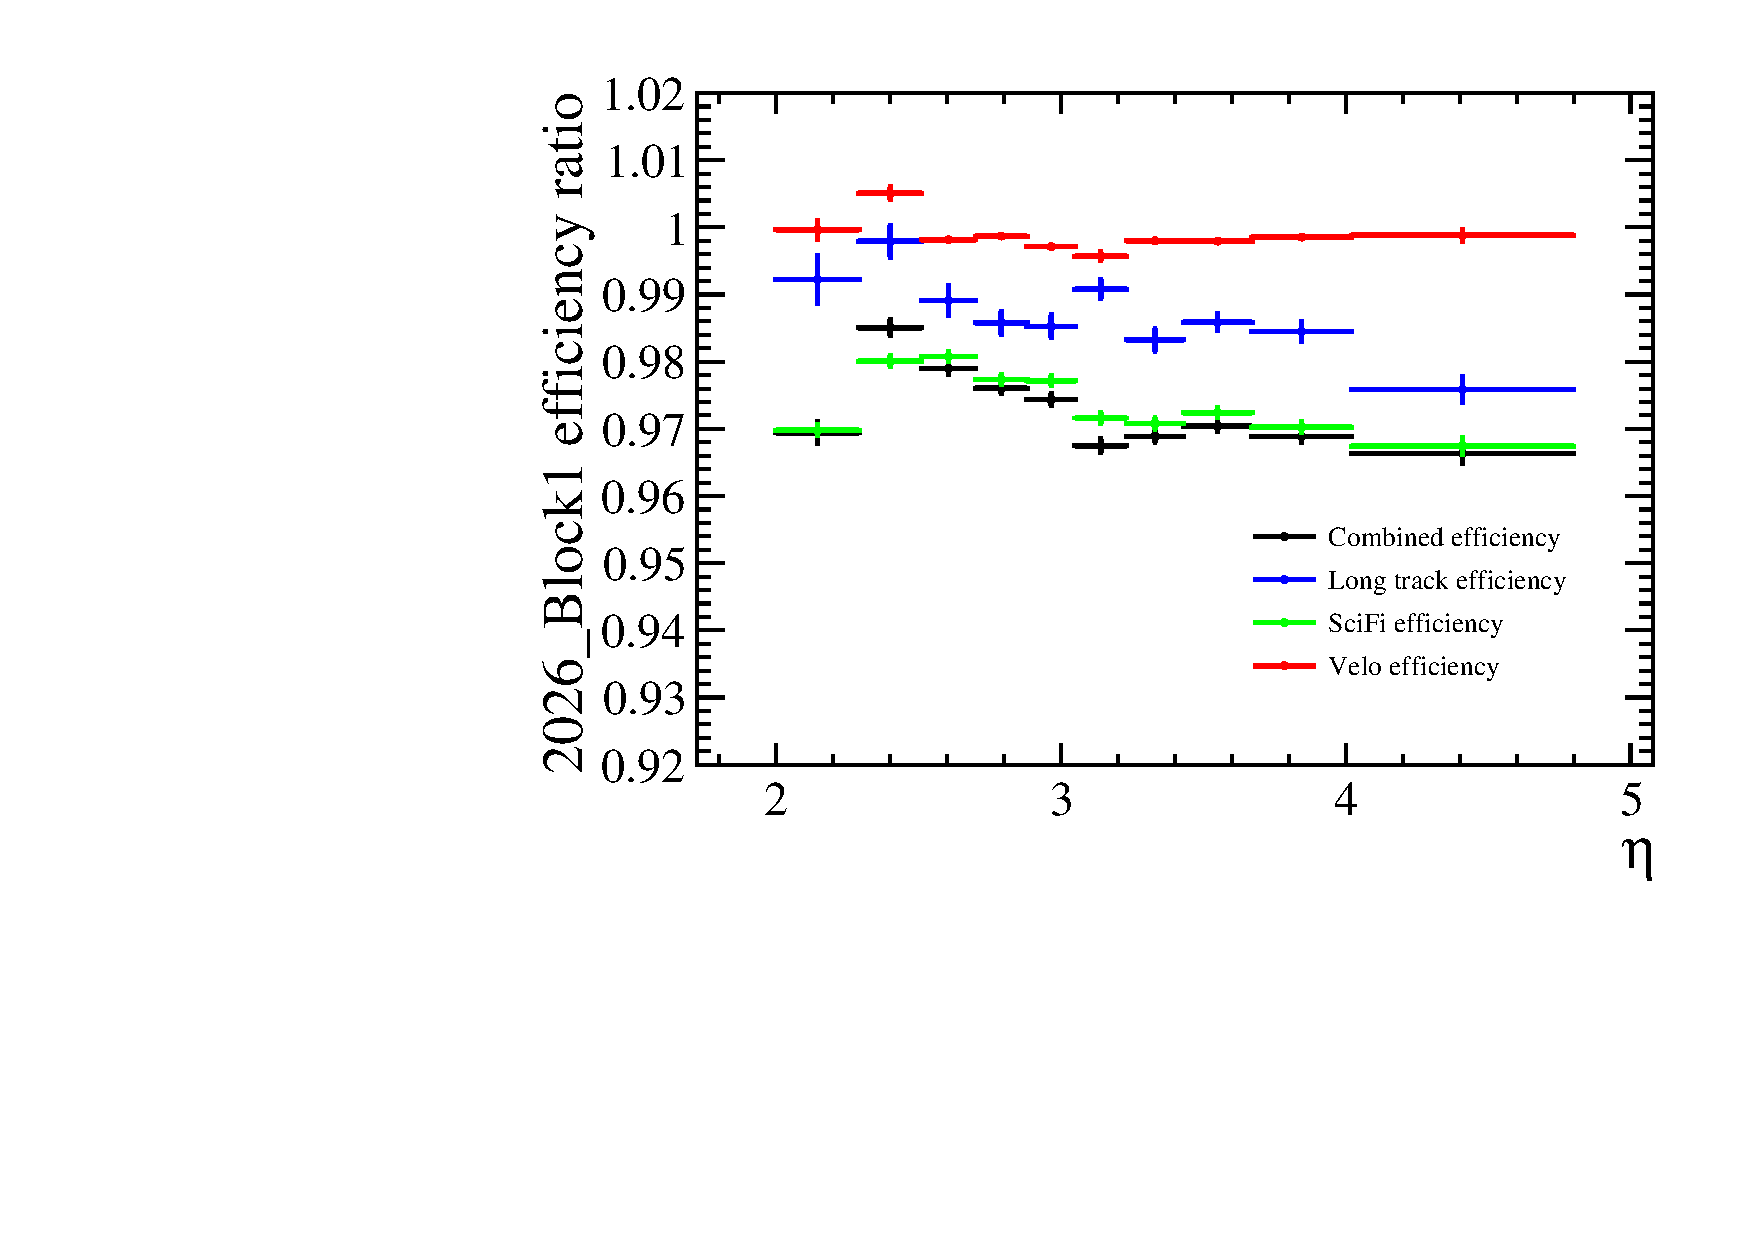
\includegraphics[width=1.0\textwidth]{Plots/trackeff_ratio_ETA_2026_Block1_2026_expected_MC_samples.pdf}
    \end{subfigure}
  \end{figure}
  {No surprises in 2026 Block 1}
\end{frame}

\begin{frame}{2026 tracking efficiency ratios}
  \vspace{0.0cm}
  {\large Comparison of tracking efficiency ratios in 2026 Block 2}
  \begin{figure}[htb]
    \centering
    \begin{subfigure}{0.5\textwidth}
      \centering
      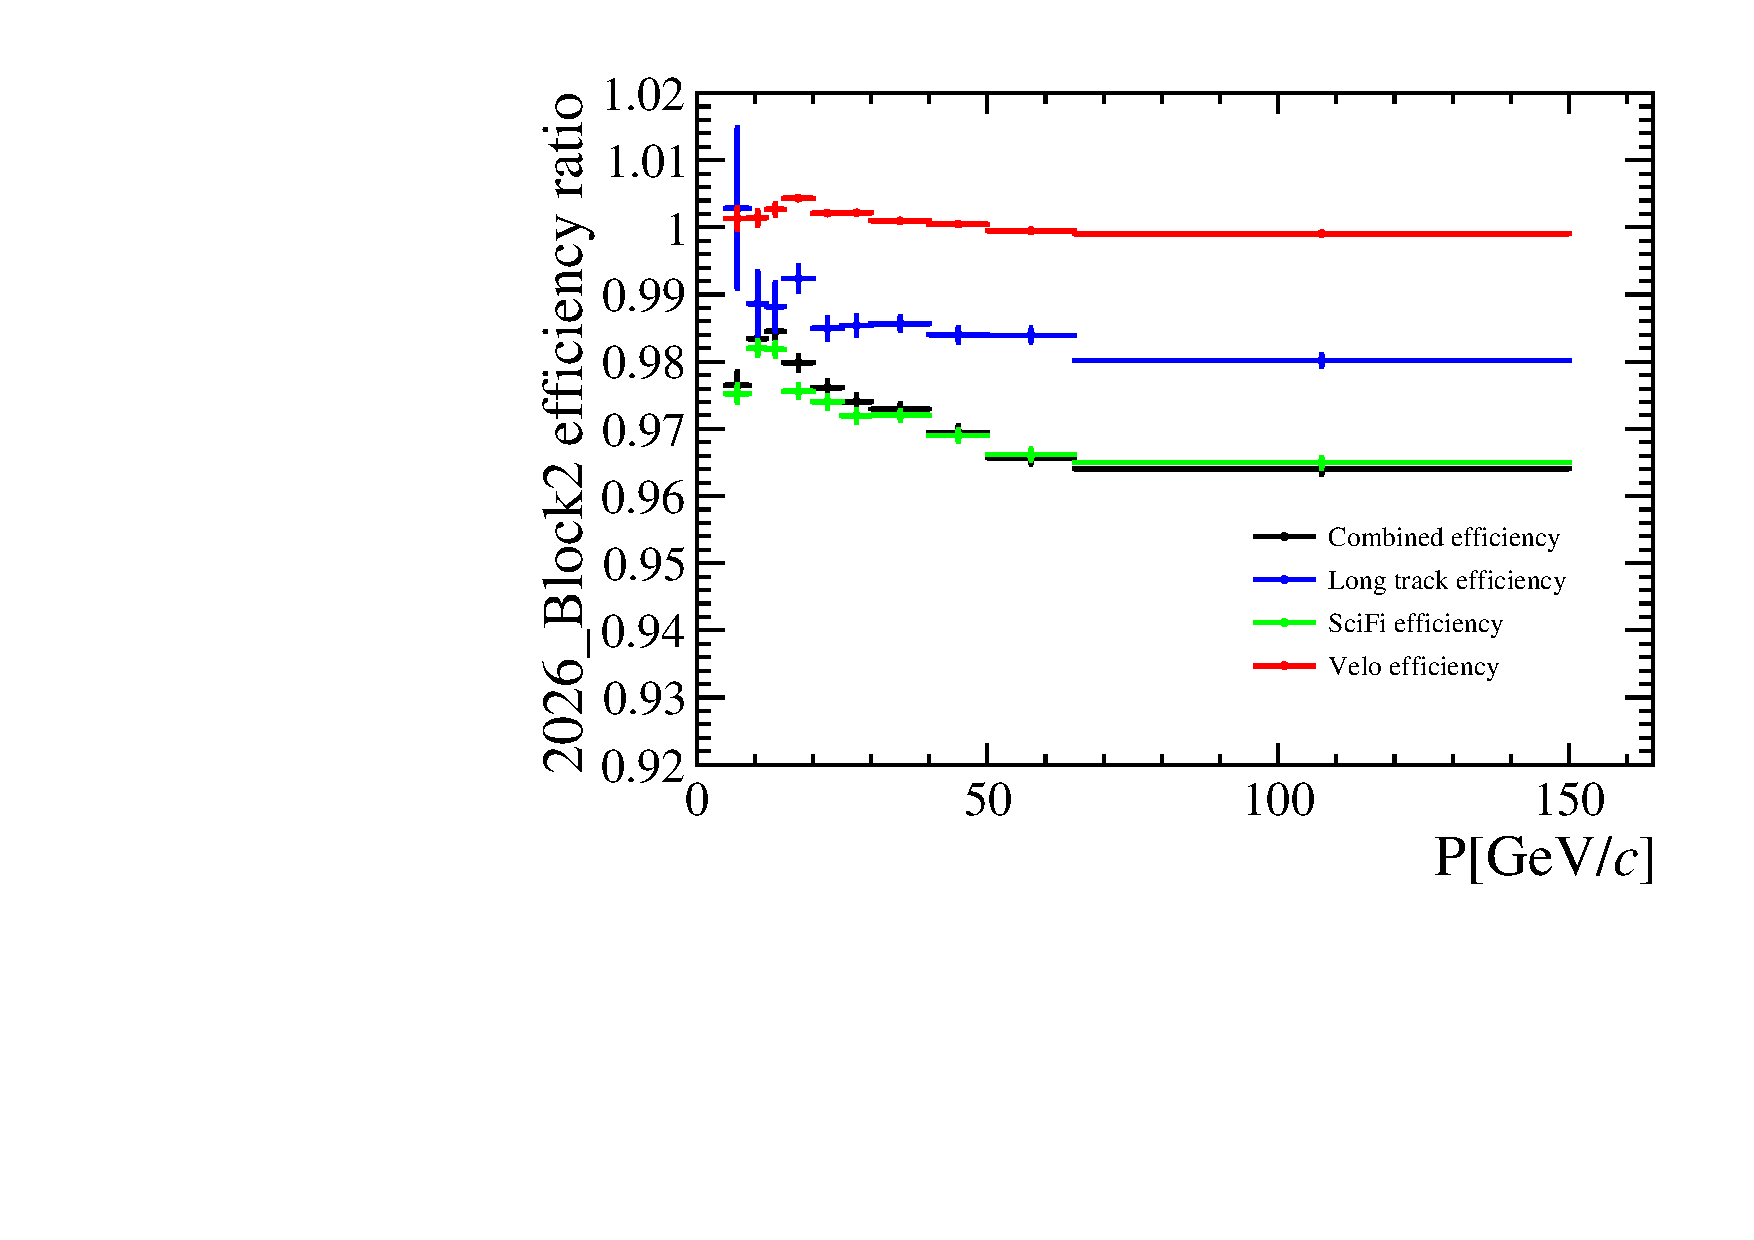
\includegraphics[width=1.0\textwidth]{Plots/trackeff_ratio_P_2026_Block2_2026_expected_MC_samples.pdf}
    \end{subfigure}%
    \begin{subfigure}{0.5\textwidth}
      \centering
      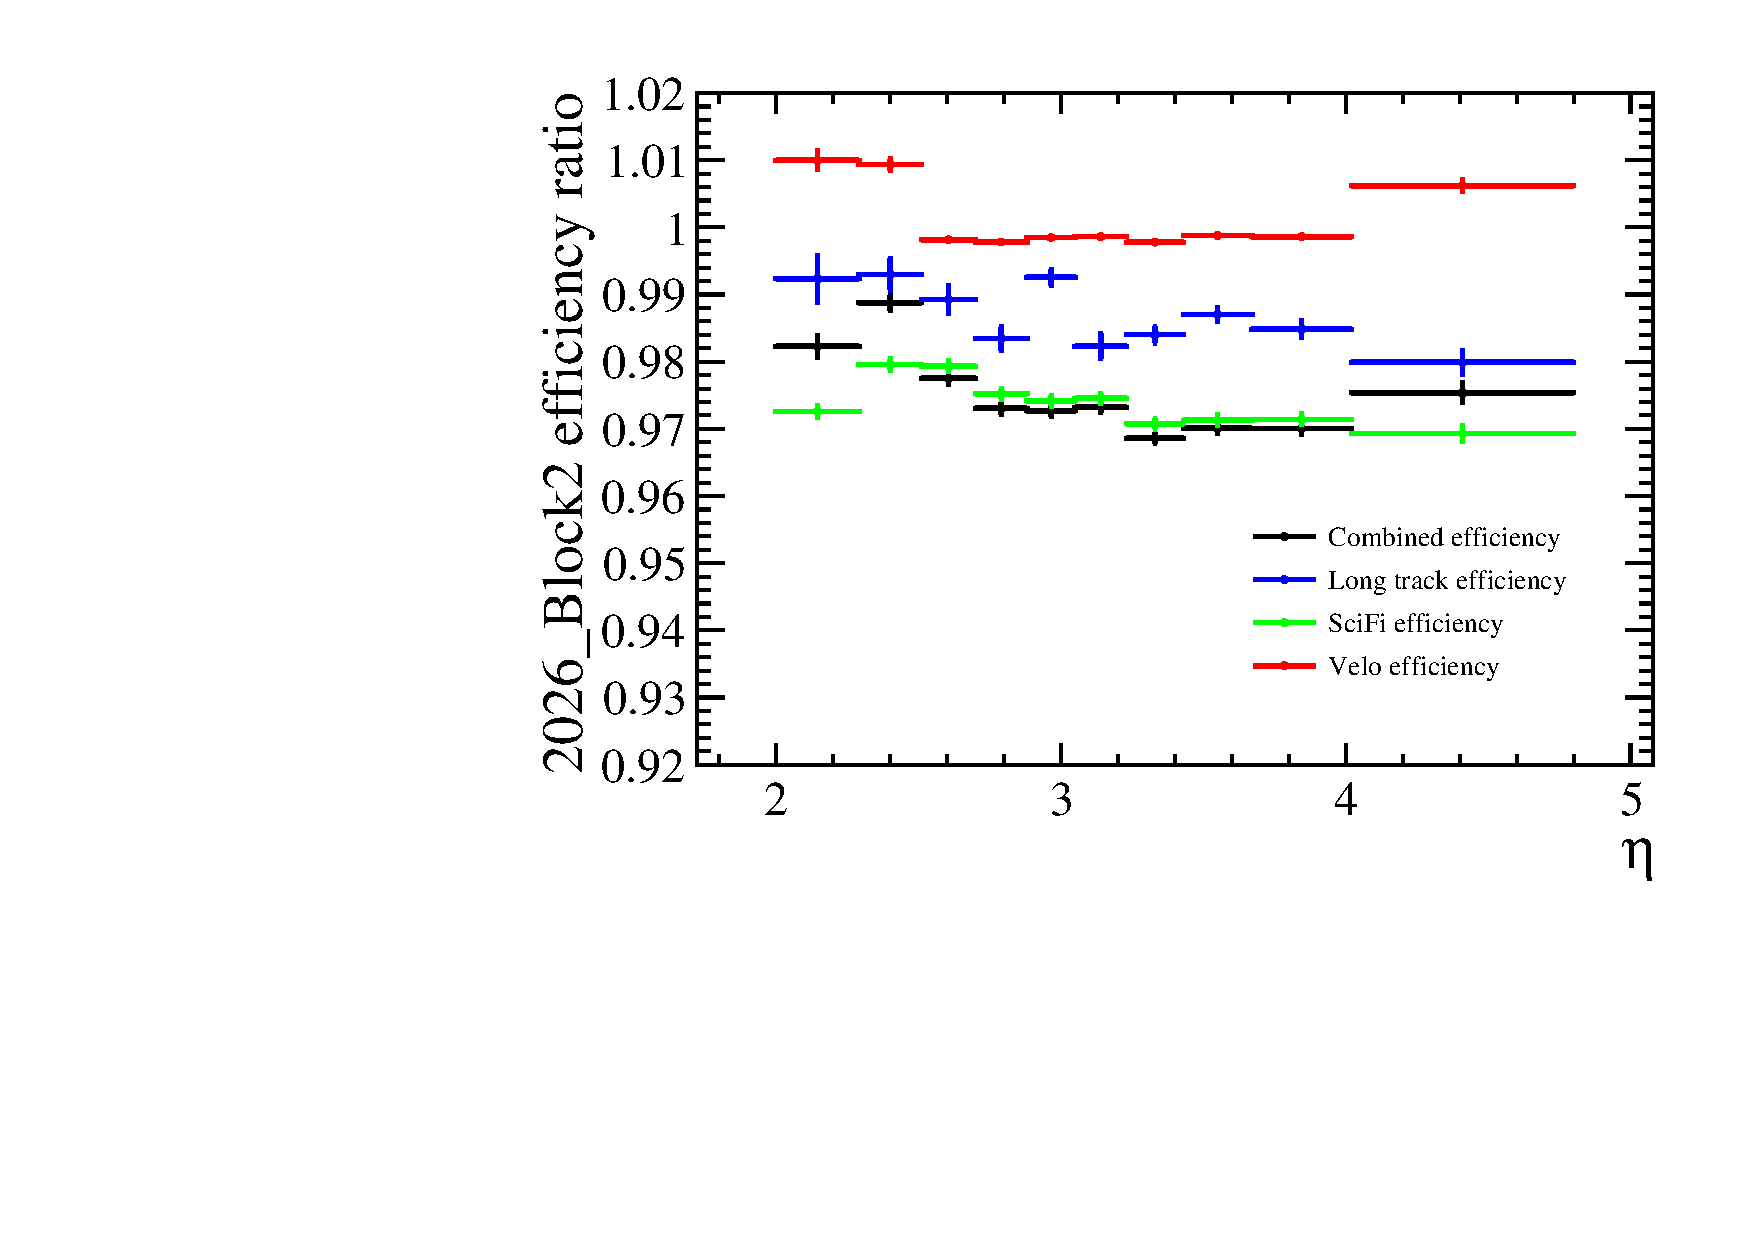
\includegraphics[width=1.0\textwidth]{Plots/trackeff_ratio_ETA_2026_Block2_2026_expected_MC_samples.pdf}
    \end{subfigure}
  \end{figure}
  {2026 Block 2 shows some discrepancies in Velo efficiencies}
\end{frame}

\begin{frame}{2026 tracking efficiency ratios}
  \vspace{0.0cm}
  {\large Comparison of tracking efficiency ratios in 2026 Block 3}
  \begin{figure}[htb]
    \centering
    \begin{subfigure}{0.5\textwidth}
      \centering
      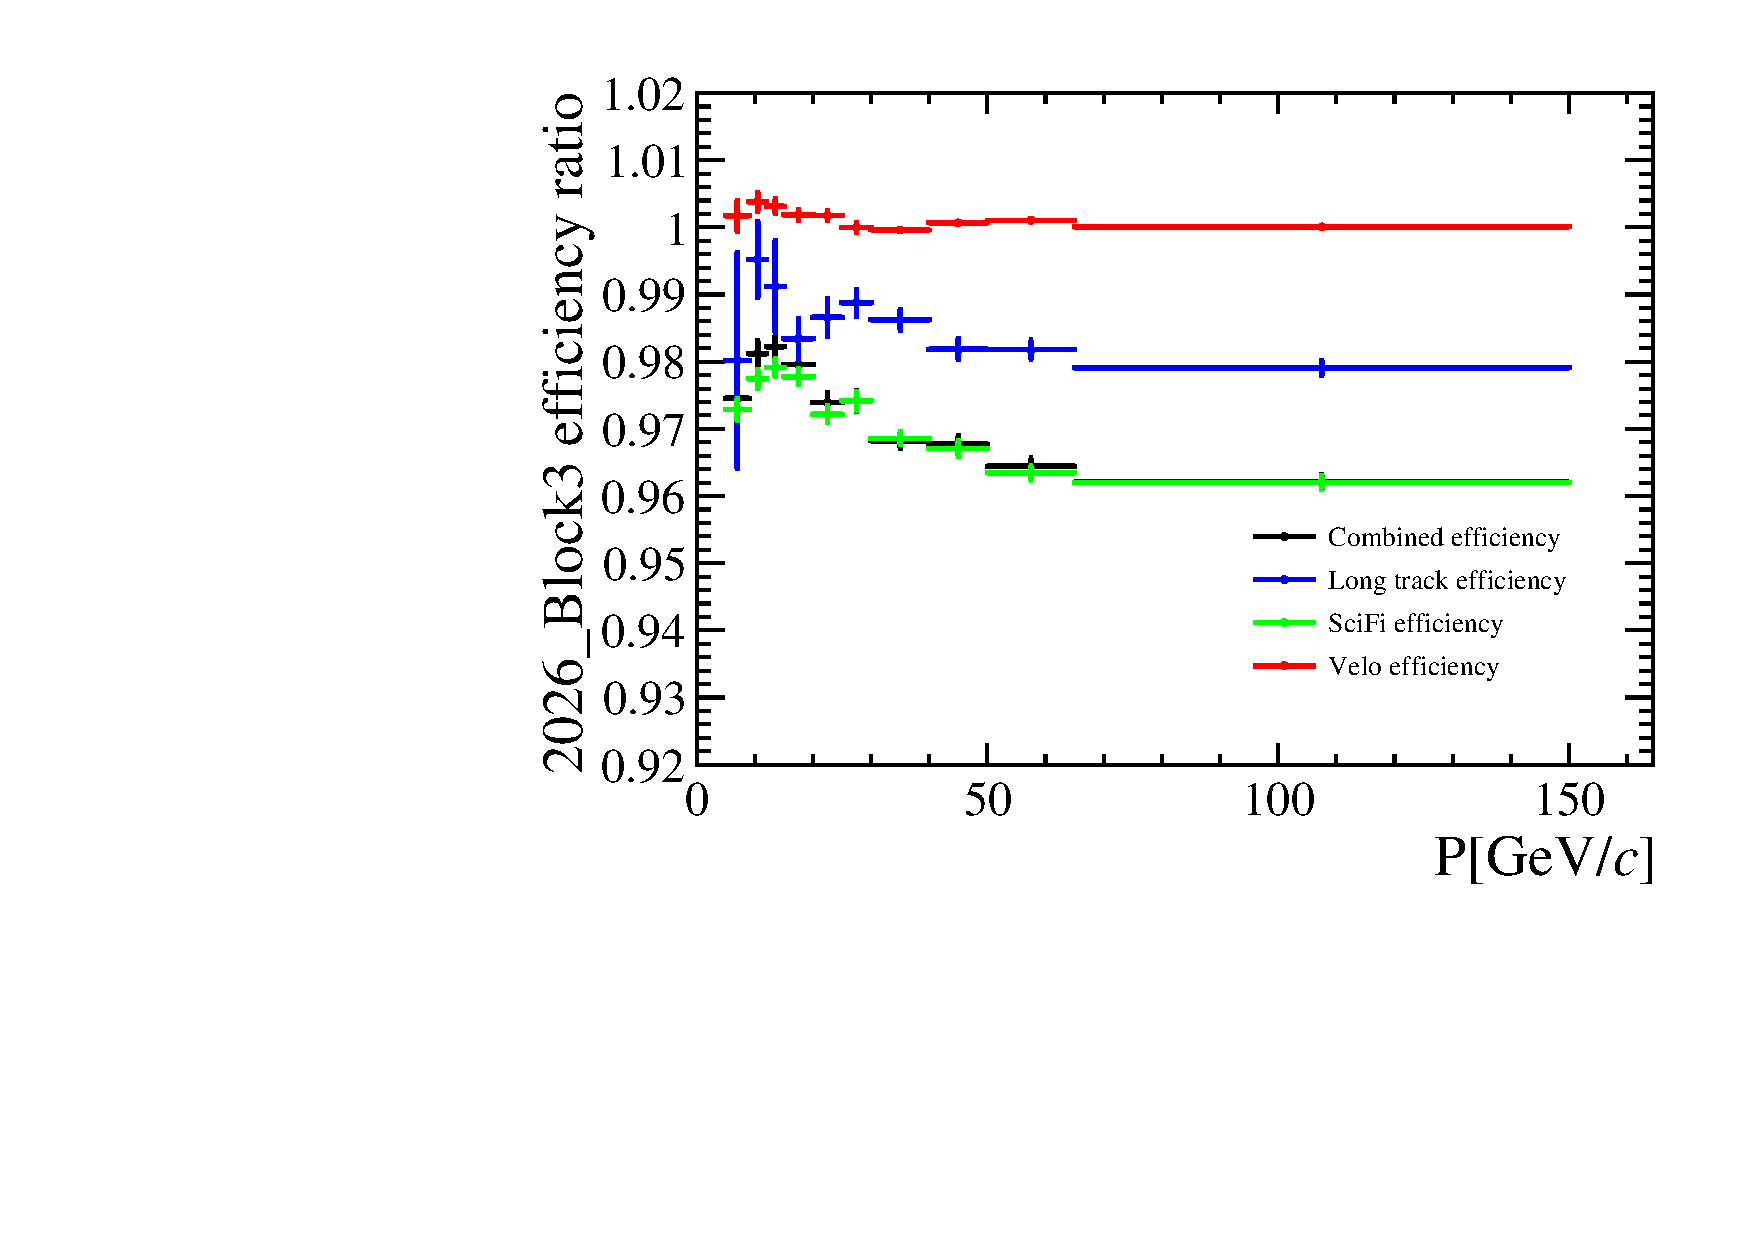
\includegraphics[width=1.0\textwidth]{Plots/trackeff_ratio_P_2026_Block3_2026_expected_MC_samples.pdf}
    \end{subfigure}%
    \begin{subfigure}{0.5\textwidth}
      \centering
      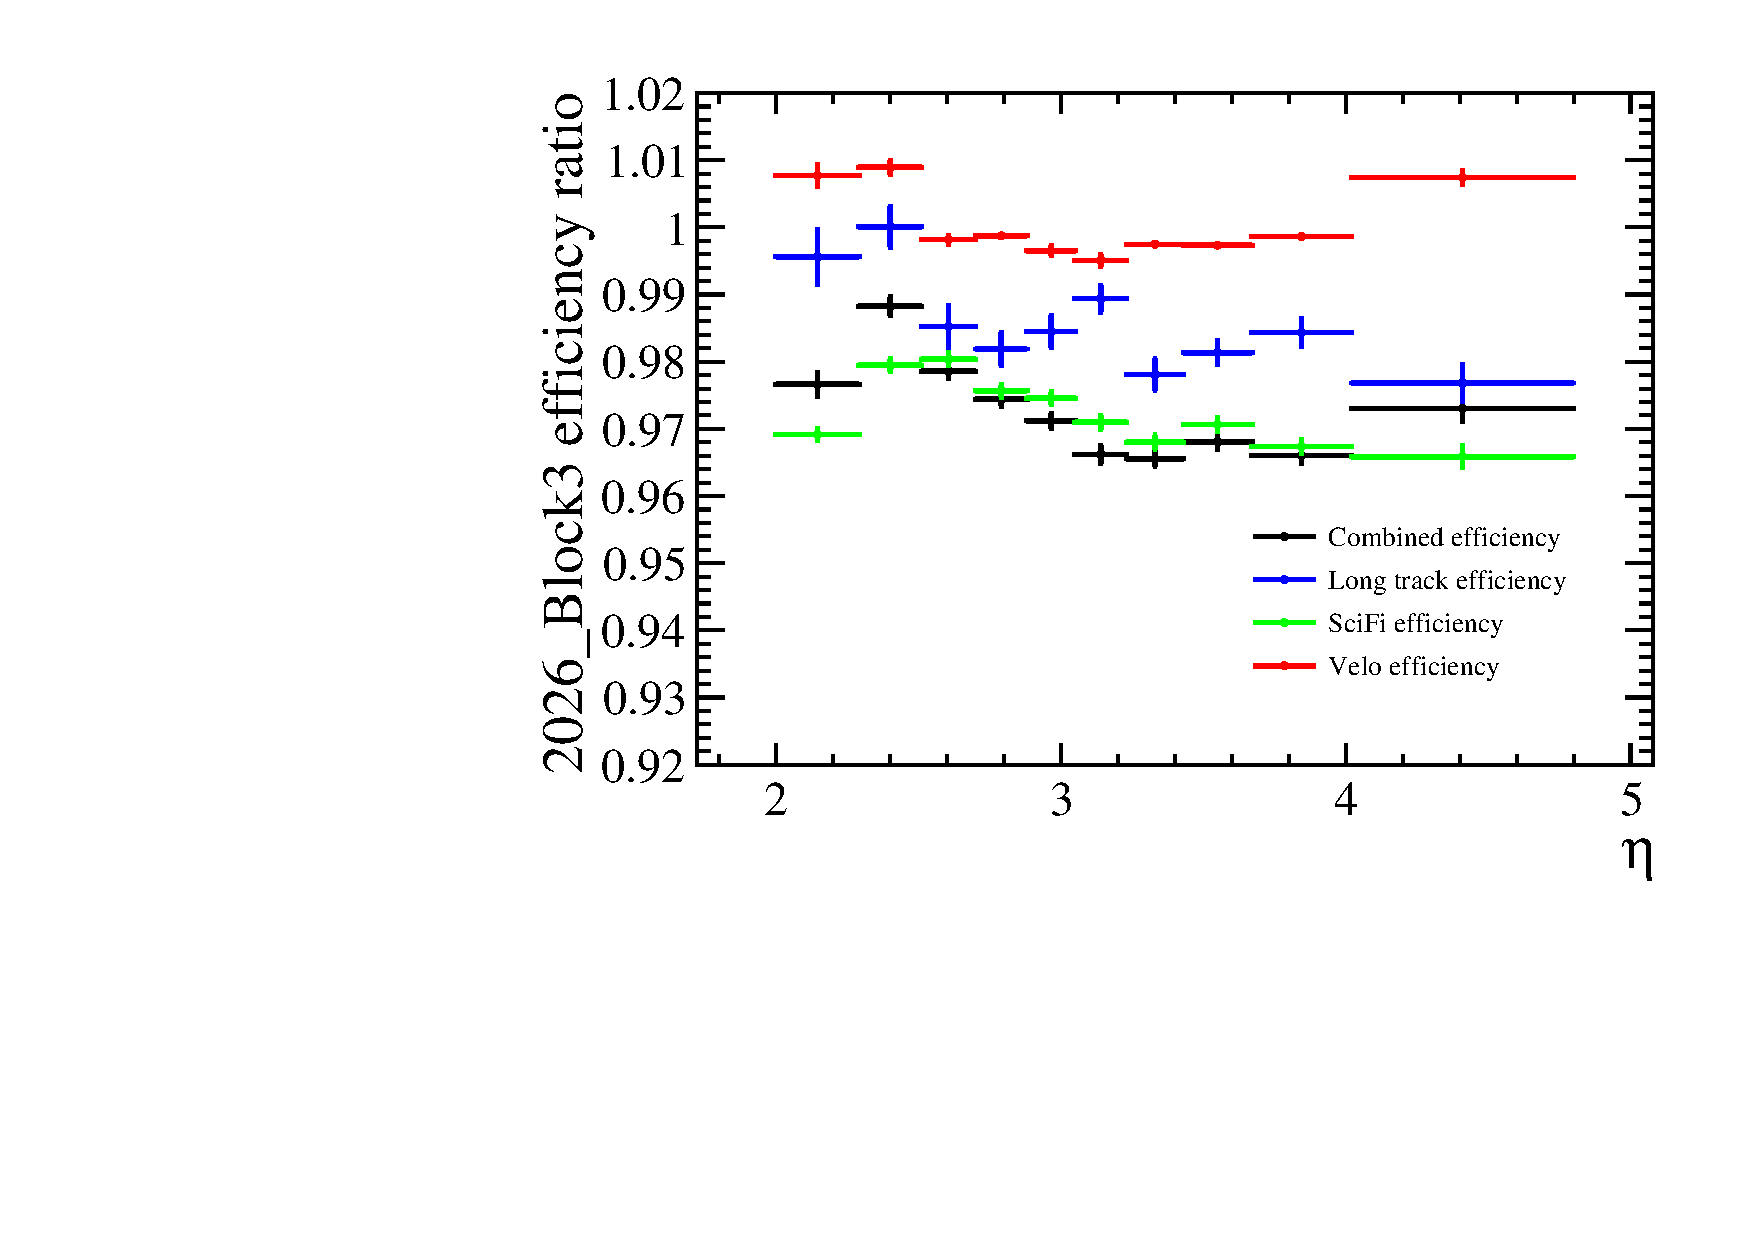
\includegraphics[width=1.0\textwidth]{Plots/trackeff_ratio_ETA_2026_Block3_2026_expected_MC_samples.pdf}
    \end{subfigure}
  \end{figure}
  {2026 Block 3 shows some discrepancies in Velo efficiencies}
\end{frame}

\begin{frame}{2026 tracking efficiency ratios}
  \vspace{0.0cm}
  {\large Comparison of tracking efficiency ratios in 2026 Block 4}
  \begin{figure}[htb]
    \centering
    \begin{subfigure}{0.5\textwidth}
      \centering
      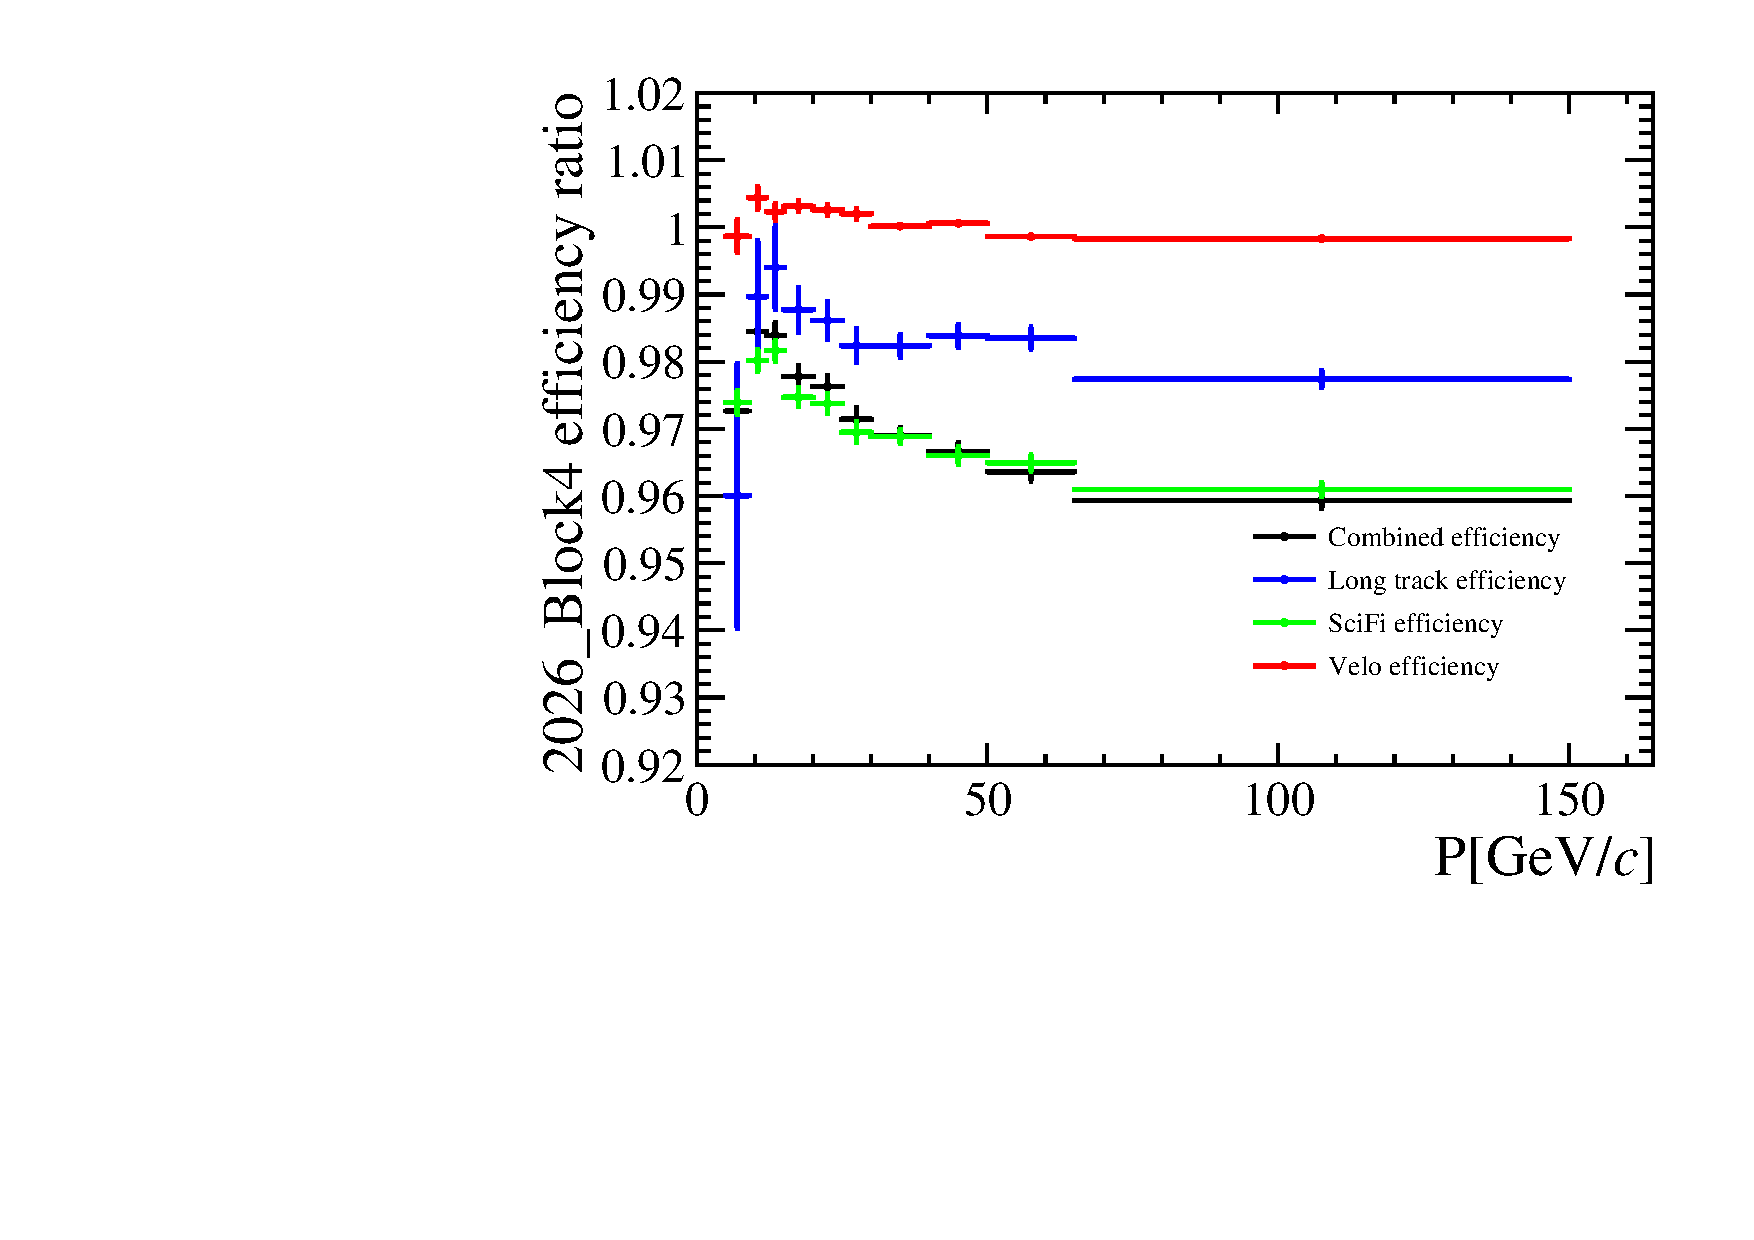
\includegraphics[width=1.0\textwidth]{Plots/trackeff_ratio_P_2026_Block4_2026_expected_MC_samples.pdf}
    \end{subfigure}%
    \begin{subfigure}{0.5\textwidth}
      \centering
      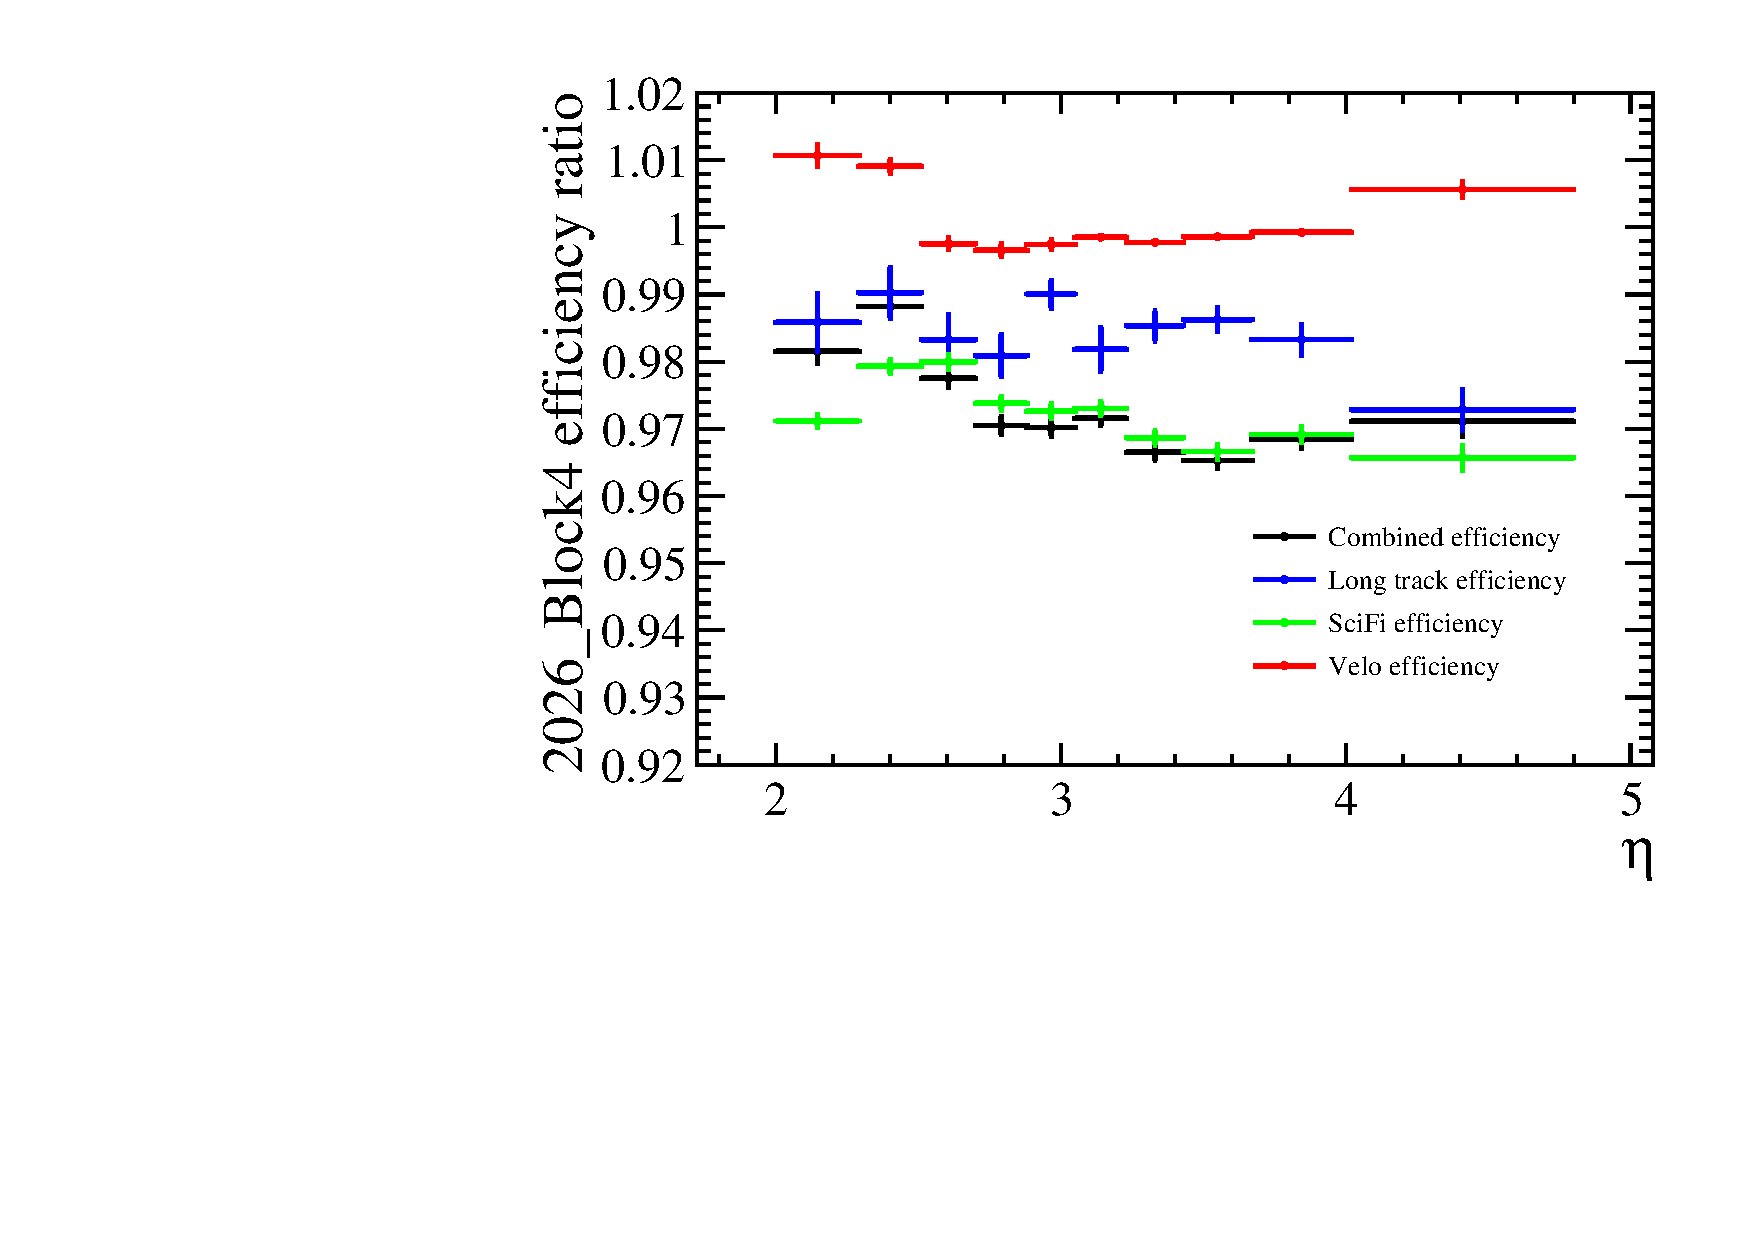
\includegraphics[width=1.0\textwidth]{Plots/trackeff_ratio_ETA_2026_Block4_2026_expected_MC_samples.pdf}
    \end{subfigure}
  \end{figure}
  {2026 Block 4 shows some discrepancies in Velo efficiencies}
\end{frame}

\begin{frame}{Multiplicity reweighting}
  \vspace{0.0cm}
  \begin{figure}[htb]
    \centering
    \begin{subfigure}{0.5\textwidth}
      \centering
      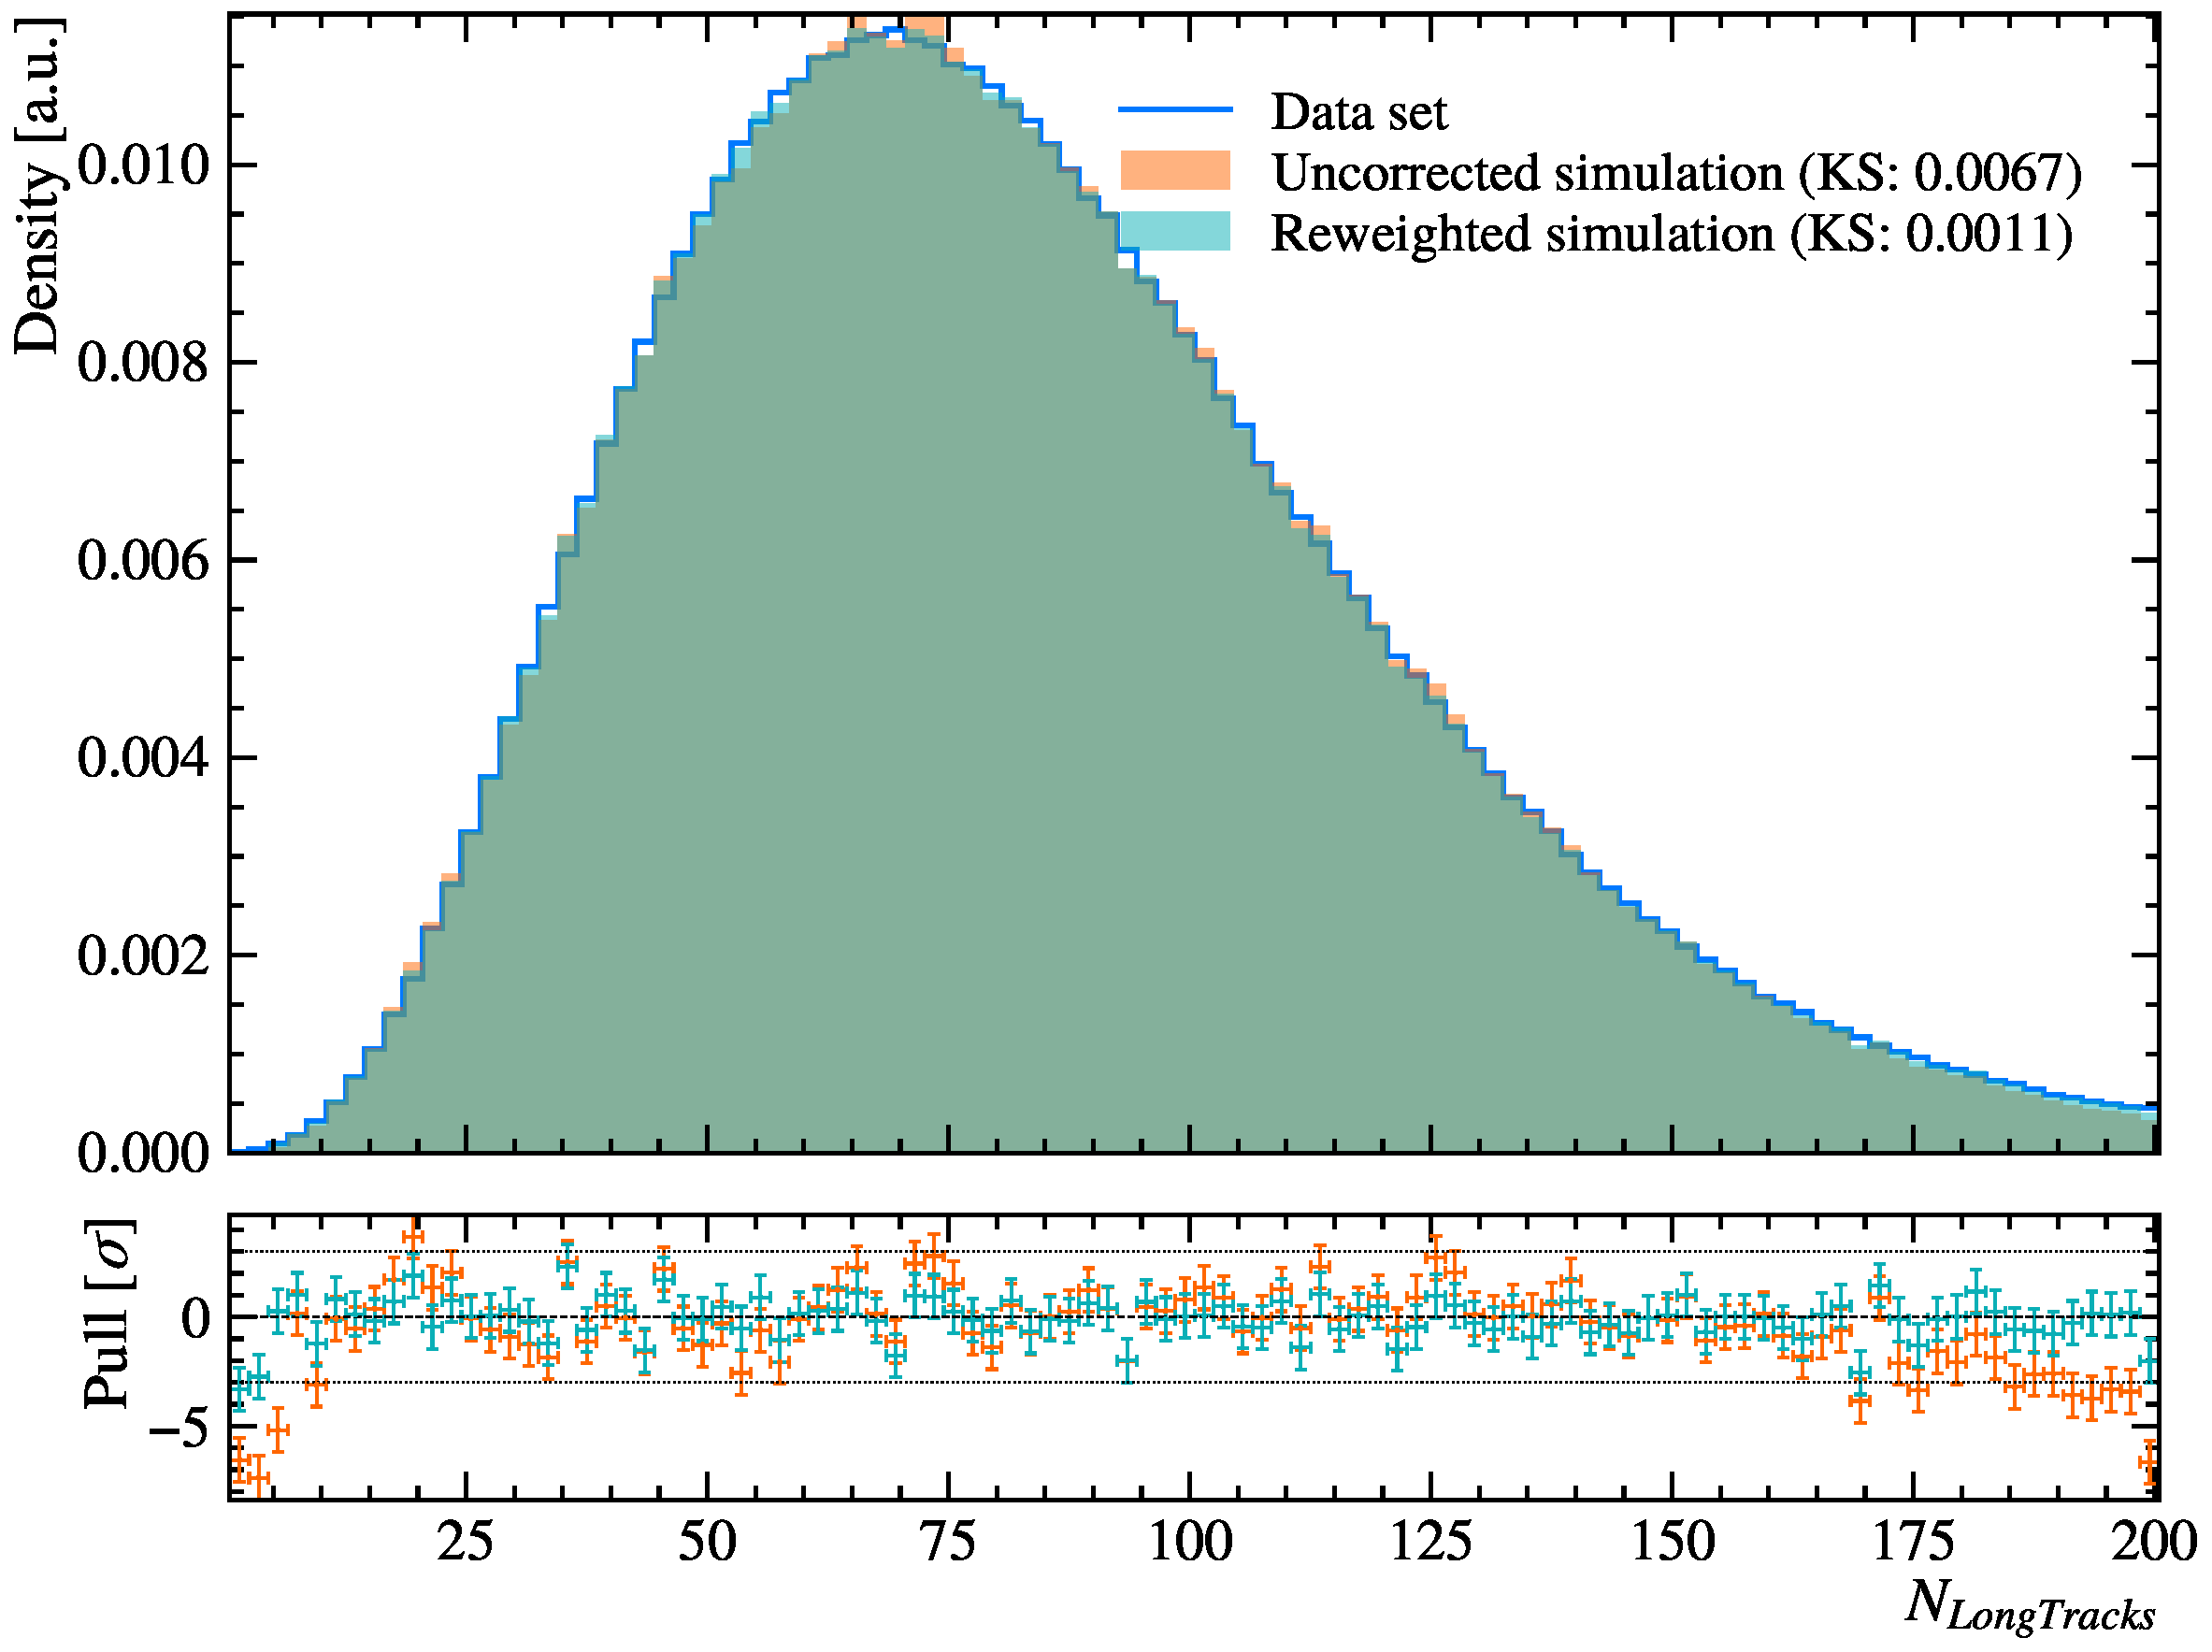
\includegraphics[width=1.0\textwidth]{Plots/VeloMuon_nLongTracks.pdf}
    \end{subfigure}%
    \begin{subfigure}{0.5\textwidth}
      \centering
      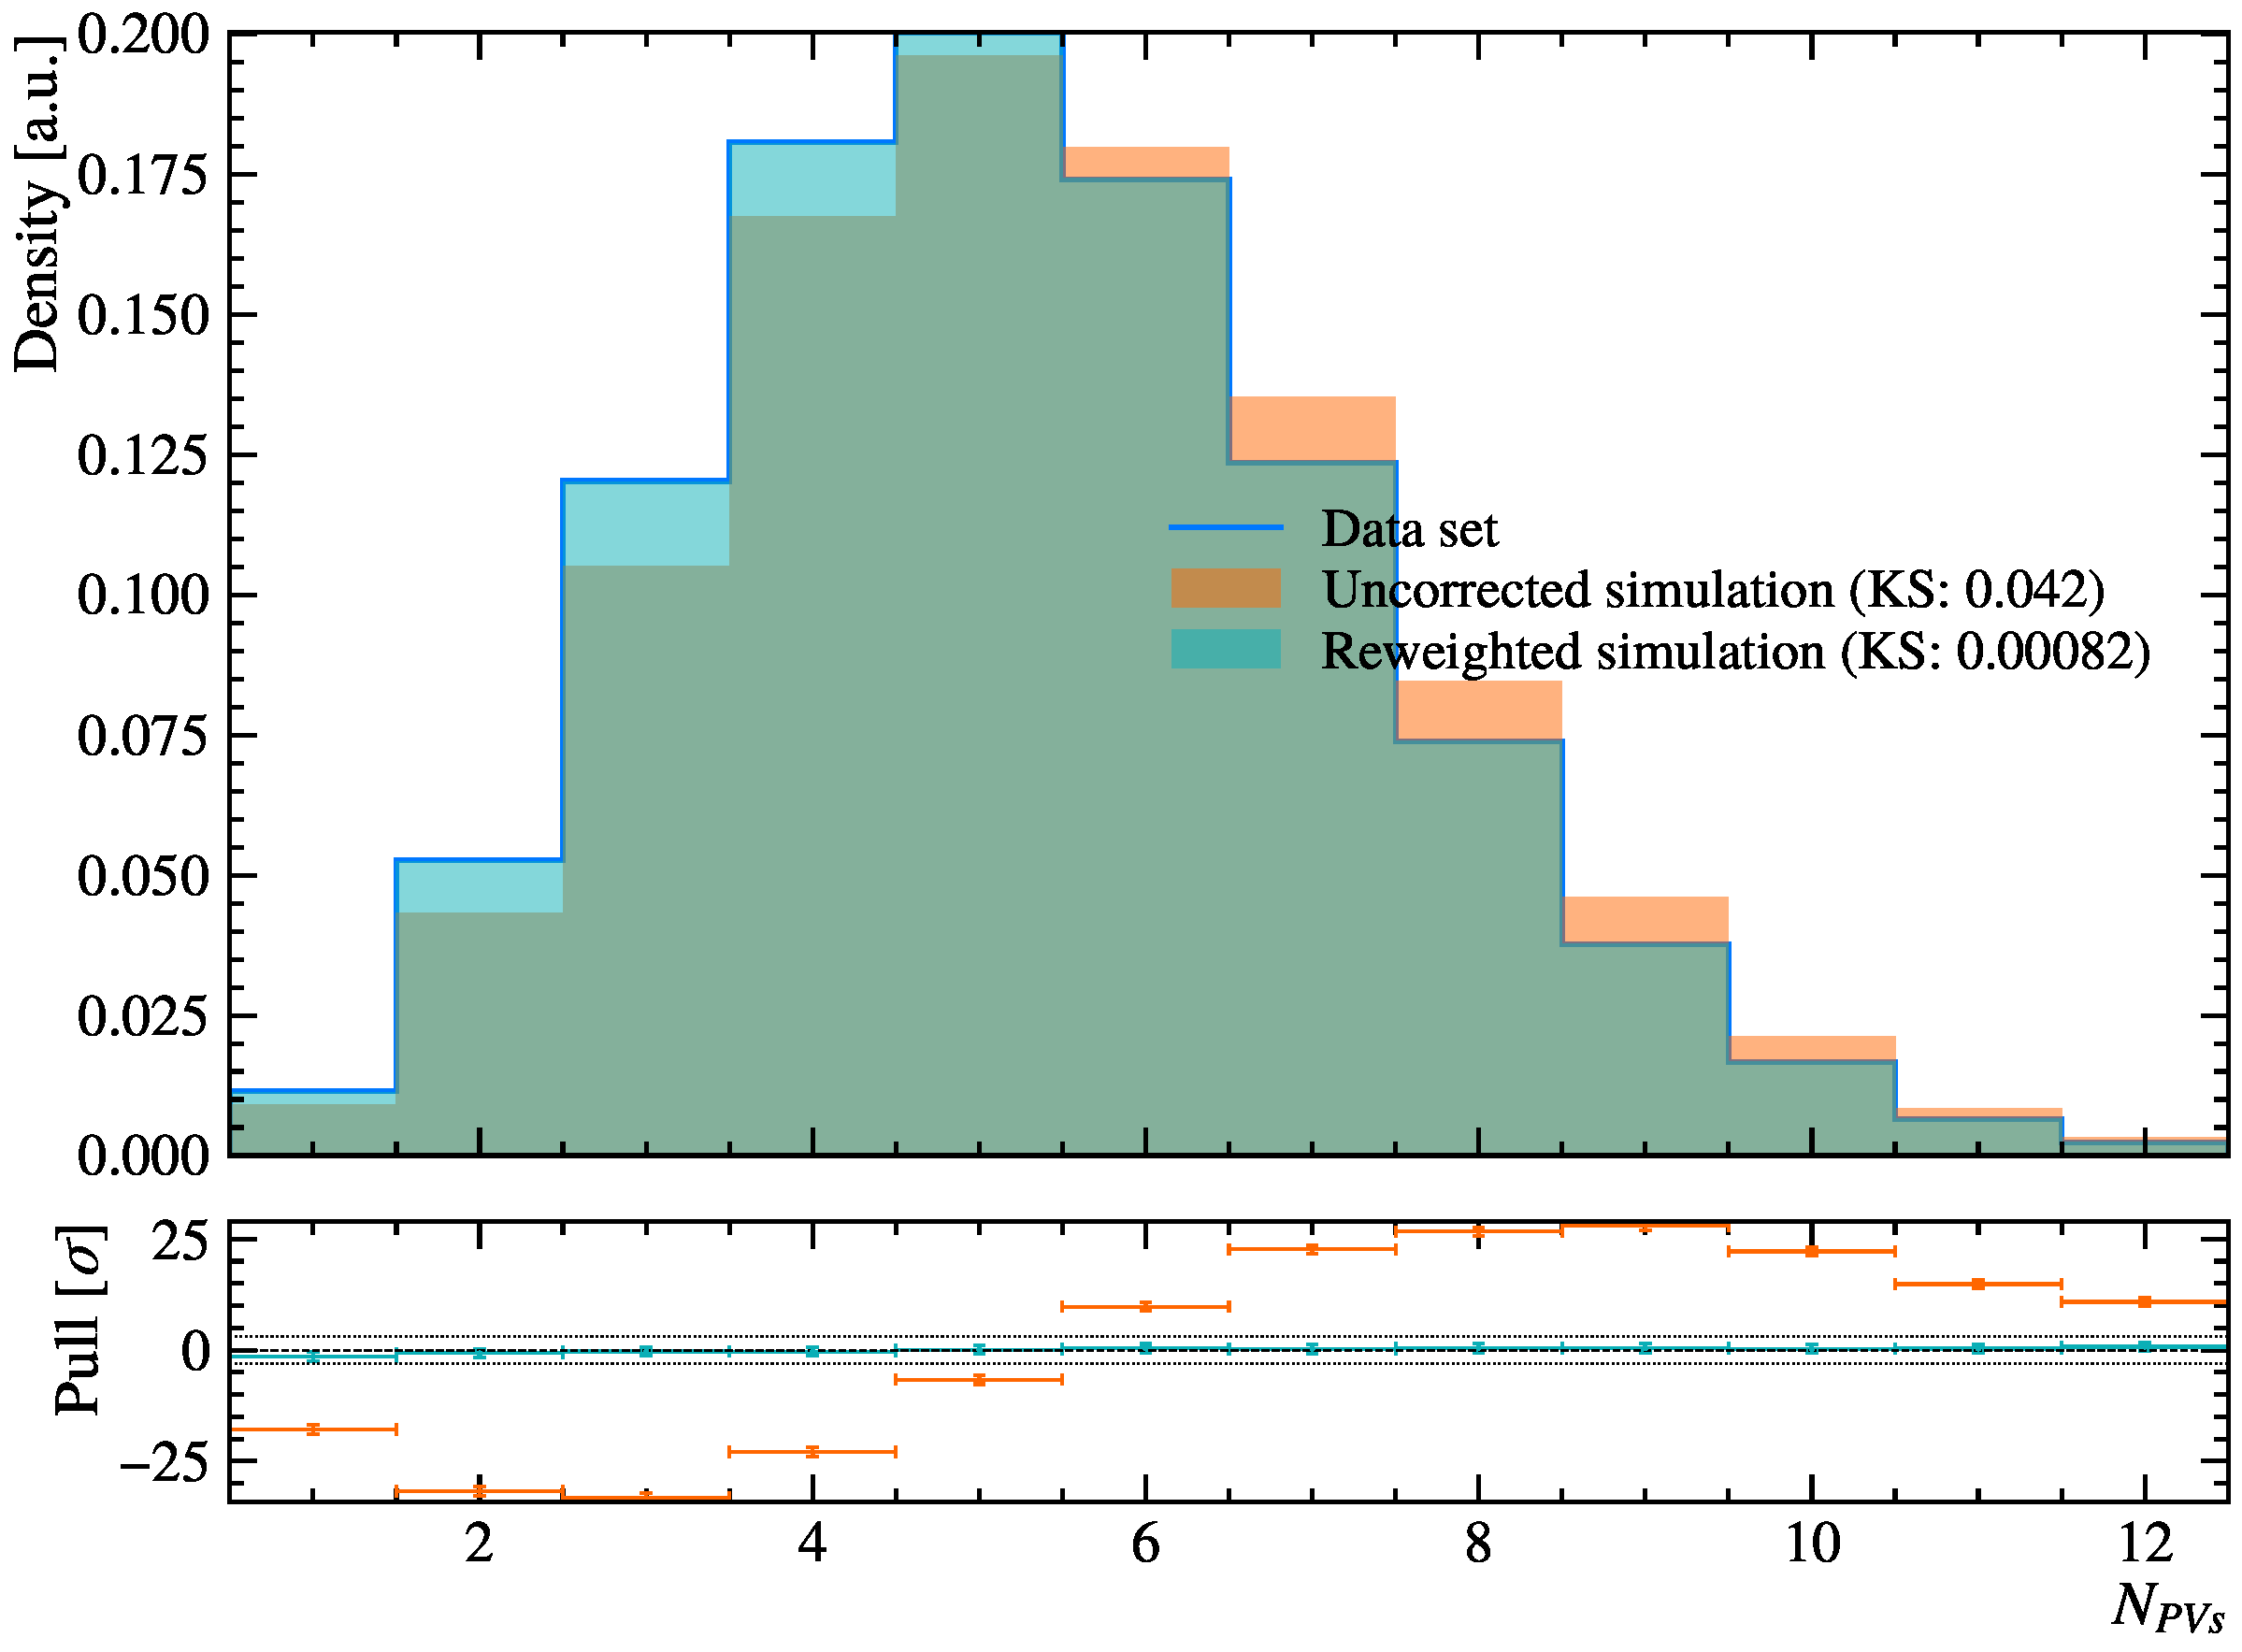
\includegraphics[width=1.0\textwidth]{Plots/VeloMuon_nPVs.pdf}
    \end{subfigure}
  \end{figure}
  \begin{itemize}
    \item{By default, reweight \texttt{nLongTracks} and \texttt{nPVs}}
    \item{Need to change from unbinned to binned fit in TrackCalib2 to get correct uncertainties}
    \item{Reweighting code in TrackCalib2 by Maurice, but with XGBoost instead of GBReweighter}
  \end{itemize}
\end{frame}

\begin{frame}{Alternative multiplicity reweighting}
  \vspace{0.0cm}
  \begin{figure}[htb]
    \centering
    \begin{subfigure}{0.5\textwidth}
      \centering
      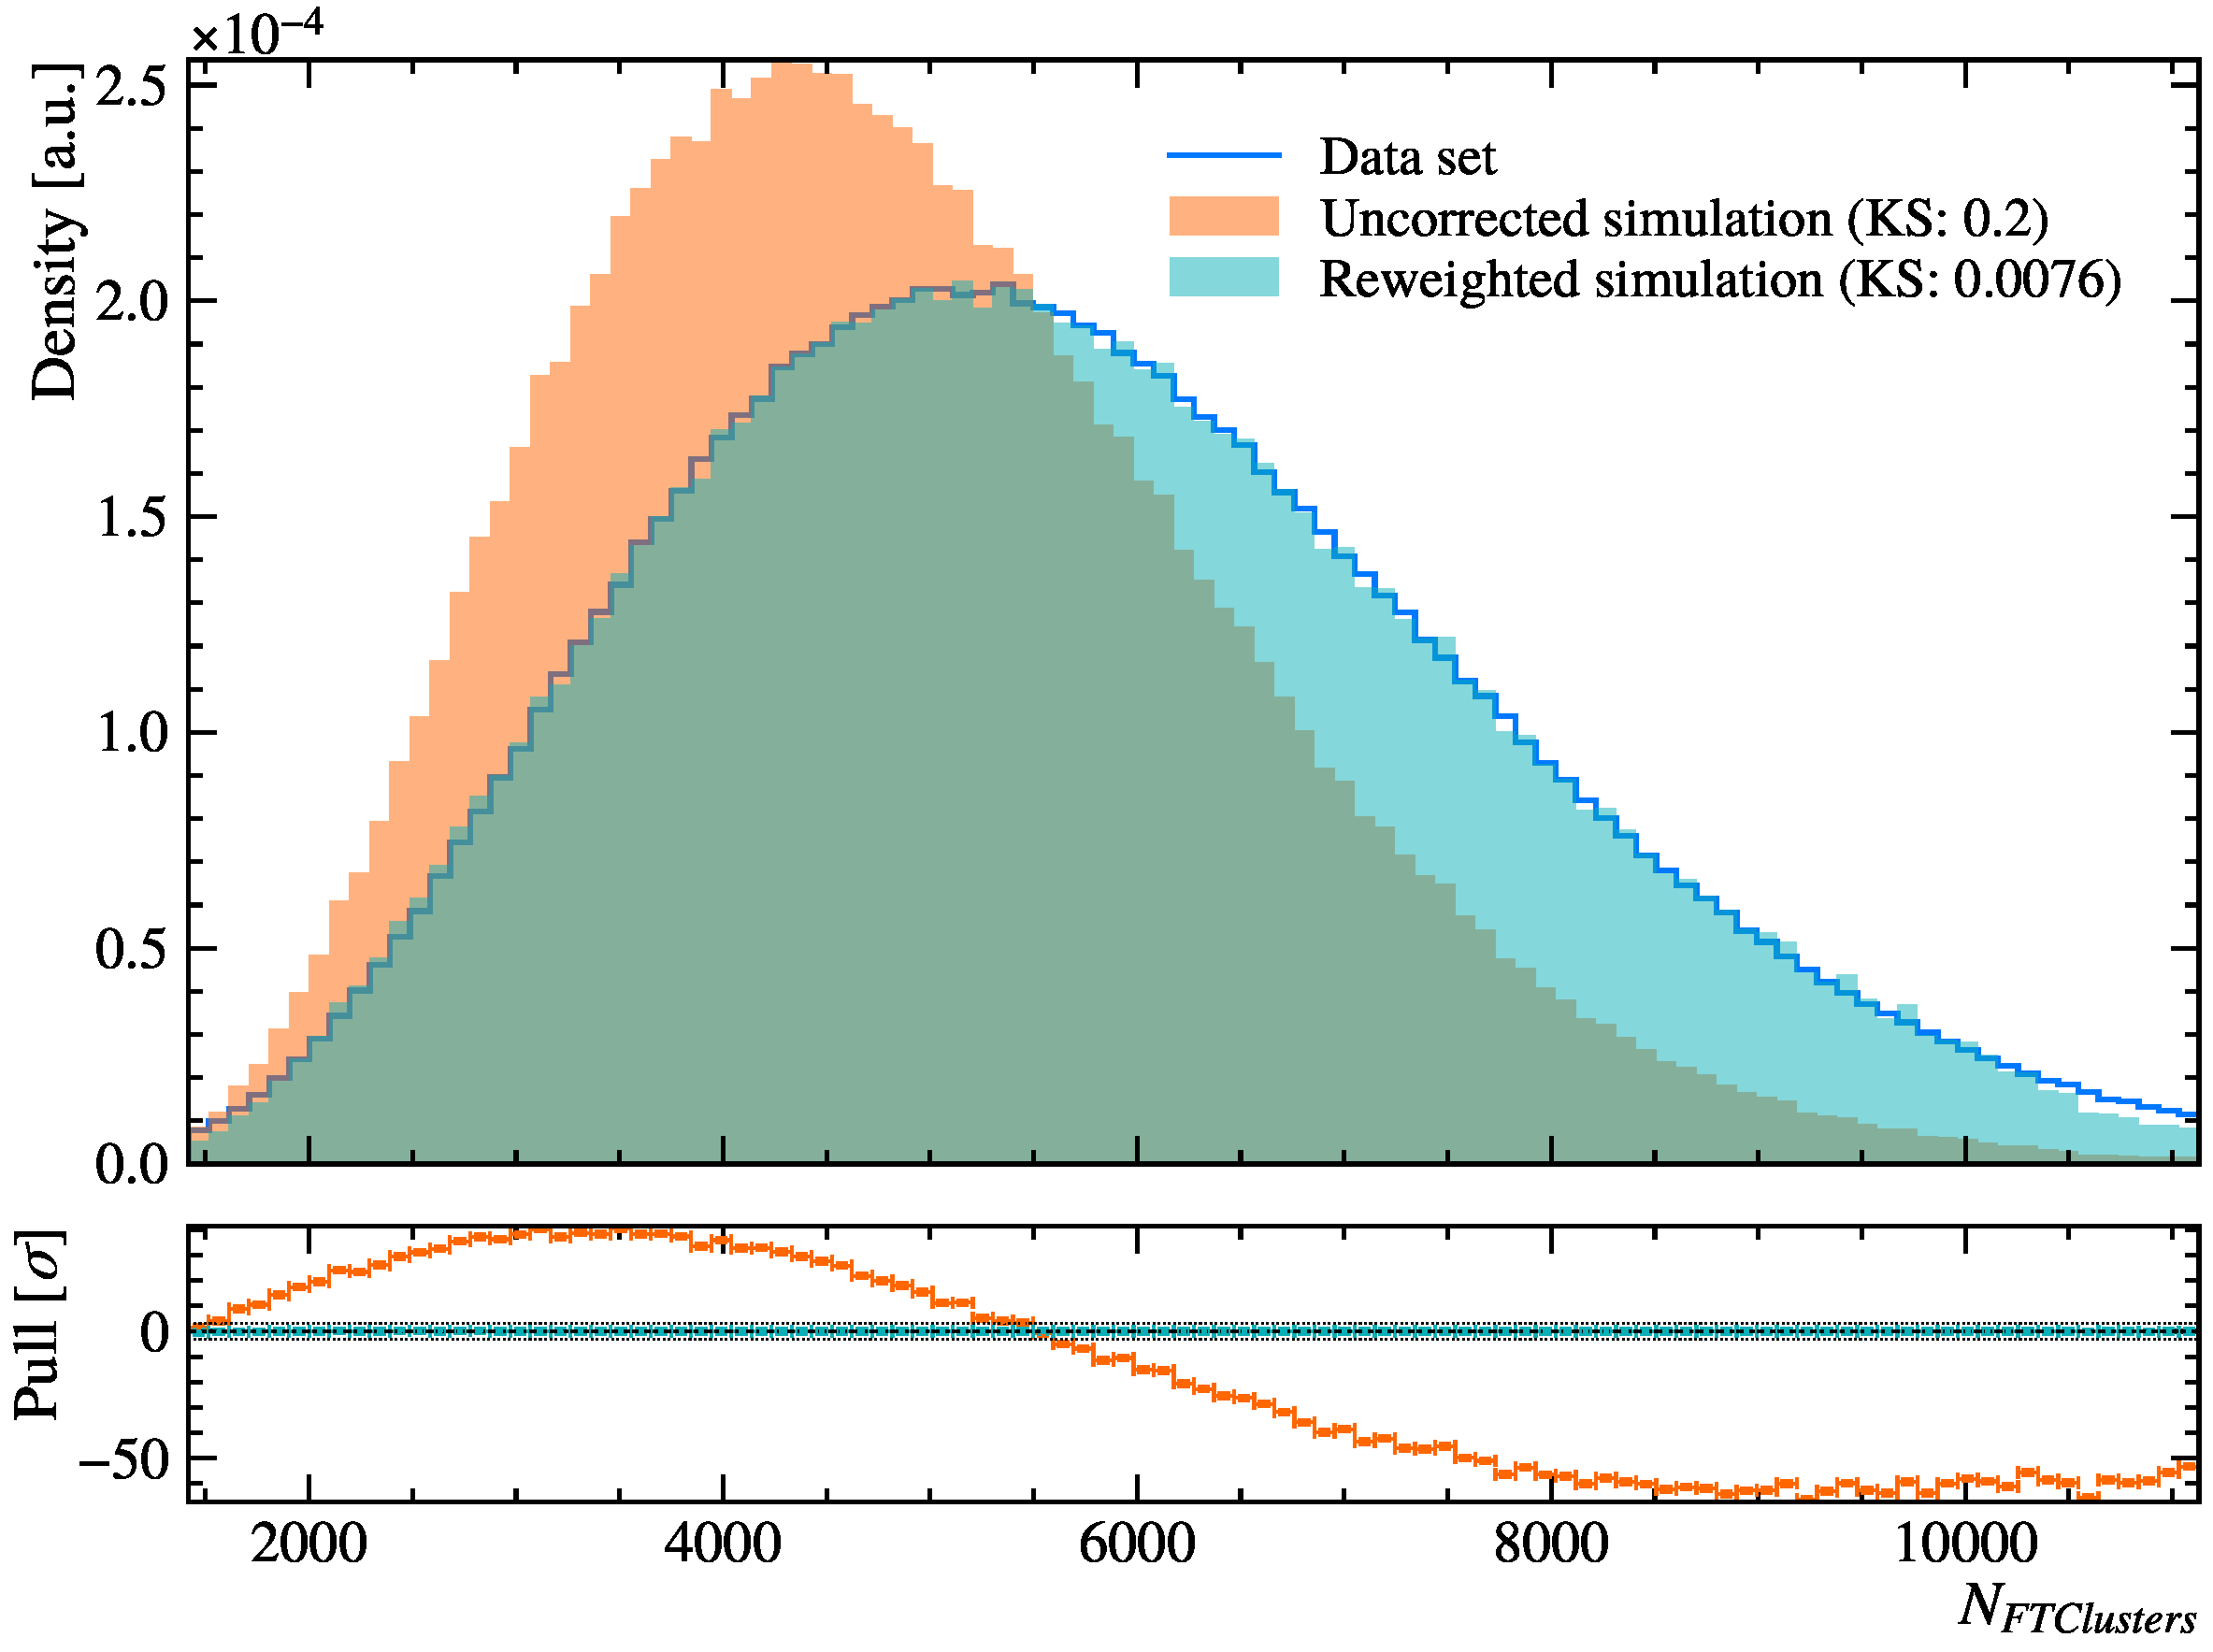
\includegraphics[width=1.0\textwidth]{Plots/VeloMuon_nFTClusters.pdf}
    \end{subfigure}
  \end{figure}
  \begin{itemize}
    \item{Reweight \texttt{nFTClusters} as an alternative}
    \item{Assign systematic due to discrepancies in multiplicity between data and MC}
    \item{Weights obtained from simple histogram}
  \end{itemize}
\end{frame}

\begin{frame}{Plan next}
  \vspace{0.0cm}
  {\large Next steps:}
  \vspace{0.2cm}
  \begin{enumerate}
    \setlength\itemsep{0.8em}
    \item{Produce correction tables for 2026 with expected MC?}
    \item{New iteration of 2024 tracking efficiencies with:}
    \begin{itemize}
      \item[-]{$\mu^\pm$, $\mu^+$, $\mu^-$ corrections}
      \item[-]{New 2D binning scheme}
      \item[-]{Full set of systematics}
    \end{itemize}
    \item{Look into block 1b MC when MC production is finished}
  \end{enumerate}
\end{frame}

\end{document}
